% Options for packages loaded elsewhere
\PassOptionsToPackage{unicode}{hyperref}
\PassOptionsToPackage{hyphens}{url}
\PassOptionsToPackage{dvipsnames,svgnames,x11names}{xcolor}
%
\documentclass[
]{article}

\usepackage{amsmath,amssymb}
\usepackage{lmodern}
\usepackage{iftex}
\ifPDFTeX
  \usepackage[T1]{fontenc}
  \usepackage[utf8]{inputenc}
  \usepackage{textcomp} % provide euro and other symbols
\else % if luatex or xetex
  \usepackage{unicode-math}
  \defaultfontfeatures{Scale=MatchLowercase}
  \defaultfontfeatures[\rmfamily]{Ligatures=TeX,Scale=1}
\fi
% Use upquote if available, for straight quotes in verbatim environments
\IfFileExists{upquote.sty}{\usepackage{upquote}}{}
\IfFileExists{microtype.sty}{% use microtype if available
  \usepackage[]{microtype}
  \UseMicrotypeSet[protrusion]{basicmath} % disable protrusion for tt fonts
}{}
\makeatletter
\@ifundefined{KOMAClassName}{% if non-KOMA class
  \IfFileExists{parskip.sty}{%
    \usepackage{parskip}
  }{% else
    \setlength{\parindent}{0pt}
    \setlength{\parskip}{6pt plus 2pt minus 1pt}}
}{% if KOMA class
  \KOMAoptions{parskip=half}}
\makeatother
\usepackage{xcolor}
\usepackage[top=30mm,left=30mm,right=20mm,bottom=20mm]{geometry}
\setlength{\emergencystretch}{3em} % prevent overfull lines
\setcounter{secnumdepth}{-\maxdimen} % remove section numbering
% Make \paragraph and \subparagraph free-standing
\ifx\paragraph\undefined\else
  \let\oldparagraph\paragraph
  \renewcommand{\paragraph}[1]{\oldparagraph{#1}\mbox{}}
\fi
\ifx\subparagraph\undefined\else
  \let\oldsubparagraph\subparagraph
  \renewcommand{\subparagraph}[1]{\oldsubparagraph{#1}\mbox{}}
\fi

\usepackage{color}
\usepackage{fancyvrb}
\newcommand{\VerbBar}{|}
\newcommand{\VERB}{\Verb[commandchars=\\\{\}]}
\DefineVerbatimEnvironment{Highlighting}{Verbatim}{commandchars=\\\{\}}
% Add ',fontsize=\small' for more characters per line
\usepackage{framed}
\definecolor{shadecolor}{RGB}{241,243,245}
\newenvironment{Shaded}{\begin{snugshade}}{\end{snugshade}}
\newcommand{\AlertTok}[1]{\textcolor[rgb]{0.68,0.00,0.00}{#1}}
\newcommand{\AnnotationTok}[1]{\textcolor[rgb]{0.37,0.37,0.37}{#1}}
\newcommand{\AttributeTok}[1]{\textcolor[rgb]{0.40,0.45,0.13}{#1}}
\newcommand{\BaseNTok}[1]{\textcolor[rgb]{0.68,0.00,0.00}{#1}}
\newcommand{\BuiltInTok}[1]{\textcolor[rgb]{0.00,0.23,0.31}{#1}}
\newcommand{\CharTok}[1]{\textcolor[rgb]{0.13,0.47,0.30}{#1}}
\newcommand{\CommentTok}[1]{\textcolor[rgb]{0.37,0.37,0.37}{#1}}
\newcommand{\CommentVarTok}[1]{\textcolor[rgb]{0.37,0.37,0.37}{\textit{#1}}}
\newcommand{\ConstantTok}[1]{\textcolor[rgb]{0.56,0.35,0.01}{#1}}
\newcommand{\ControlFlowTok}[1]{\textcolor[rgb]{0.00,0.23,0.31}{#1}}
\newcommand{\DataTypeTok}[1]{\textcolor[rgb]{0.68,0.00,0.00}{#1}}
\newcommand{\DecValTok}[1]{\textcolor[rgb]{0.68,0.00,0.00}{#1}}
\newcommand{\DocumentationTok}[1]{\textcolor[rgb]{0.37,0.37,0.37}{\textit{#1}}}
\newcommand{\ErrorTok}[1]{\textcolor[rgb]{0.68,0.00,0.00}{#1}}
\newcommand{\ExtensionTok}[1]{\textcolor[rgb]{0.00,0.23,0.31}{#1}}
\newcommand{\FloatTok}[1]{\textcolor[rgb]{0.68,0.00,0.00}{#1}}
\newcommand{\FunctionTok}[1]{\textcolor[rgb]{0.28,0.35,0.67}{#1}}
\newcommand{\ImportTok}[1]{\textcolor[rgb]{0.00,0.46,0.62}{#1}}
\newcommand{\InformationTok}[1]{\textcolor[rgb]{0.37,0.37,0.37}{#1}}
\newcommand{\KeywordTok}[1]{\textcolor[rgb]{0.00,0.23,0.31}{#1}}
\newcommand{\NormalTok}[1]{\textcolor[rgb]{0.00,0.23,0.31}{#1}}
\newcommand{\OperatorTok}[1]{\textcolor[rgb]{0.37,0.37,0.37}{#1}}
\newcommand{\OtherTok}[1]{\textcolor[rgb]{0.00,0.23,0.31}{#1}}
\newcommand{\PreprocessorTok}[1]{\textcolor[rgb]{0.68,0.00,0.00}{#1}}
\newcommand{\RegionMarkerTok}[1]{\textcolor[rgb]{0.00,0.23,0.31}{#1}}
\newcommand{\SpecialCharTok}[1]{\textcolor[rgb]{0.37,0.37,0.37}{#1}}
\newcommand{\SpecialStringTok}[1]{\textcolor[rgb]{0.13,0.47,0.30}{#1}}
\newcommand{\StringTok}[1]{\textcolor[rgb]{0.13,0.47,0.30}{#1}}
\newcommand{\VariableTok}[1]{\textcolor[rgb]{0.07,0.07,0.07}{#1}}
\newcommand{\VerbatimStringTok}[1]{\textcolor[rgb]{0.13,0.47,0.30}{#1}}
\newcommand{\WarningTok}[1]{\textcolor[rgb]{0.37,0.37,0.37}{\textit{#1}}}

\providecommand{\tightlist}{%
  \setlength{\itemsep}{0pt}\setlength{\parskip}{0pt}}\usepackage{longtable,booktabs,array}
\usepackage{calc} % for calculating minipage widths
% Correct order of tables after \paragraph or \subparagraph
\usepackage{etoolbox}
\makeatletter
\patchcmd\longtable{\par}{\if@noskipsec\mbox{}\fi\par}{}{}
\makeatother
% Allow footnotes in longtable head/foot
\IfFileExists{footnotehyper.sty}{\usepackage{footnotehyper}}{\usepackage{footnote}}
\makesavenoteenv{longtable}
\usepackage{graphicx}
\makeatletter
\def\maxwidth{\ifdim\Gin@nat@width>\linewidth\linewidth\else\Gin@nat@width\fi}
\def\maxheight{\ifdim\Gin@nat@height>\textheight\textheight\else\Gin@nat@height\fi}
\makeatother
% Scale images if necessary, so that they will not overflow the page
% margins by default, and it is still possible to overwrite the defaults
% using explicit options in \includegraphics[width, height, ...]{}
\setkeys{Gin}{width=\maxwidth,height=\maxheight,keepaspectratio}
% Set default figure placement to htbp
\makeatletter
\def\fps@figure{htbp}
\makeatother
\newlength{\cslhangindent}
\setlength{\cslhangindent}{1.5em}
\newlength{\csllabelwidth}
\setlength{\csllabelwidth}{3em}
\newlength{\cslentryspacingunit} % times entry-spacing
\setlength{\cslentryspacingunit}{\parskip}
\newenvironment{CSLReferences}[2] % #1 hanging-ident, #2 entry spacing
 {% don't indent paragraphs
  \setlength{\parindent}{0pt}
  % turn on hanging indent if param 1 is 1
  \ifodd #1
  \let\oldpar\par
  \def\par{\hangindent=\cslhangindent\oldpar}
  \fi
  % set entry spacing
  \setlength{\parskip}{#2\cslentryspacingunit}
 }%
 {}
\usepackage{calc}
\newcommand{\CSLBlock}[1]{#1\hfill\break}
\newcommand{\CSLLeftMargin}[1]{\parbox[t]{\csllabelwidth}{#1}}
\newcommand{\CSLRightInline}[1]{\parbox[t]{\linewidth - \csllabelwidth}{#1}\break}
\newcommand{\CSLIndent}[1]{\hspace{\cslhangindent}#1}

\makeatletter
\makeatother
\makeatletter
\makeatother
\makeatletter
\@ifpackageloaded{caption}{}{\usepackage{caption}}
\AtBeginDocument{%
\ifdefined\contentsname
  \renewcommand*\contentsname{Table of contents}
\else
  \newcommand\contentsname{Table of contents}
\fi
\ifdefined\listfigurename
  \renewcommand*\listfigurename{List of Figures}
\else
  \newcommand\listfigurename{List of Figures}
\fi
\ifdefined\listtablename
  \renewcommand*\listtablename{List of Tables}
\else
  \newcommand\listtablename{List of Tables}
\fi
\ifdefined\figurename
  \renewcommand*\figurename{Figure}
\else
  \newcommand\figurename{Figure}
\fi
\ifdefined\tablename
  \renewcommand*\tablename{Table}
\else
  \newcommand\tablename{Table}
\fi
}
\@ifpackageloaded{float}{}{\usepackage{float}}
\floatstyle{ruled}
\@ifundefined{c@chapter}{\newfloat{codelisting}{h}{lop}}{\newfloat{codelisting}{h}{lop}[chapter]}
\floatname{codelisting}{Listing}
\newcommand*\listoflistings{\listof{codelisting}{List of Listings}}
\makeatother
\makeatletter
\@ifpackageloaded{caption}{}{\usepackage{caption}}
\@ifpackageloaded{subcaption}{}{\usepackage{subcaption}}
\makeatother
\makeatletter
\@ifpackageloaded{tcolorbox}{}{\usepackage[many]{tcolorbox}}
\makeatother
\makeatletter
\@ifundefined{shadecolor}{\definecolor{shadecolor}{rgb}{.97, .97, .97}}
\makeatother
\makeatletter
\makeatother
\ifLuaTeX
  \usepackage{selnolig}  % disable illegal ligatures
\fi
\IfFileExists{bookmark.sty}{\usepackage{bookmark}}{\usepackage{hyperref}}
\IfFileExists{xurl.sty}{\usepackage{xurl}}{} % add URL line breaks if available
\urlstyle{same} % disable monospaced font for URLs
\hypersetup{
  pdftitle={Estimação},
  colorlinks=true,
  linkcolor={blue},
  filecolor={Maroon},
  citecolor={Blue},
  urlcolor={Blue},
  pdfcreator={LaTeX via pandoc}}

\title{Estimação}
\author{}
\date{}

\begin{document}
\maketitle
\ifdefined\Shaded\renewenvironment{Shaded}{\begin{tcolorbox}[interior hidden, breakable, borderline west={3pt}{0pt}{shadecolor}, enhanced, boxrule=0pt, frame hidden, sharp corners]}{\end{tcolorbox}}\fi

\hypertarget{carregando-base-de-dados}{%
\subsection{Carregando base de dados}\label{carregando-base-de-dados}}

\begin{Shaded}
\begin{Highlighting}[]
\NormalTok{data }\OtherTok{=}\NormalTok{ utils}\SpecialCharTok{::}\FunctionTok{read.csv}\NormalTok{(}\AttributeTok{file =} \StringTok{"pense2019\_microdados.csv"}\NormalTok{)}
\end{Highlighting}
\end{Shaded}

\hypertarget{limpando-os-dados}{%
\subsection{Limpando os dados}\label{limpando-os-dados}}

\begin{Shaded}
\begin{Highlighting}[]
\FunctionTok{library}\NormalTok{(janitor)}

\CommentTok{\# Selecionando variáveis importantes e filtrando registros válidos.}

\NormalTok{clean\_data }\OtherTok{=}\NormalTok{ janitor}\SpecialCharTok{::}\FunctionTok{clean\_names}\NormalTok{(data) }\SpecialCharTok{|\textgreater{}}
\NormalTok{  dplyr}\SpecialCharTok{::}\FunctionTok{rename}\NormalTok{(}
    \AttributeTok{tabagismo =}\NormalTok{ b04003,}
    \AttributeTok{sexo =}\NormalTok{ b01001a,}
    \AttributeTok{idade =}\NormalTok{ b01003,}
    \AttributeTok{mes\_aniversario =}\NormalTok{ b01004,}
    \AttributeTok{ano\_nascimento =}\NormalTok{ b01005,}
    \AttributeTok{cor =}\NormalTok{ b01002,}
    \AttributeTok{celular =}\NormalTok{ b01014,}
    \AttributeTok{computador =}\NormalTok{ b01015b,}
    \AttributeTok{internet =}\NormalTok{ b01016,}
    \AttributeTok{carro =}\NormalTok{ b01017,}
    \AttributeTok{moto =}\NormalTok{ b01018a,}
    \AttributeTok{banheiro =}\NormalTok{ b01019a,}
    \AttributeTok{escolaridade\_mae =}\NormalTok{ b01008b,}
    \AttributeTok{ano\_escolar =}\NormalTok{ b01021a,}
    \AttributeTok{atividade\_fisica =}\NormalTok{ b03006b,}
    \AttributeTok{bebida\_alcoolica =}\NormalTok{ b05004a,}
    \AttributeTok{dias\_tristes =}\NormalTok{ b12005,}
    \AttributeTok{sentimento\_corpo =}\NormalTok{ b11007,}
    \AttributeTok{frequencia\_pais\_problemas =}\NormalTok{ b07004,}
    \AttributeTok{amigos\_fumaram =}\NormalTok{ b04016,}
    \AttributeTok{pais\_fumam =}\NormalTok{ b04006b,}
    \AttributeTok{escola\_frequencia\_violencia\_colegas =}\NormalTok{ b07012,}
    \AttributeTok{escola\_acesso\_internet =}\NormalTok{ e01p09a,}
    \AttributeTok{escola\_atividades\_fisicas =}\NormalTok{ e01p74,}
    \AttributeTok{escola\_prevencao\_uso\_tabaco =}\NormalTok{ e01p8506,}
    \AttributeTok{escola\_consumo\_cigarro\_professores =}\NormalTok{ e01p26a,}
\NormalTok{  ) }\SpecialCharTok{|\textgreater{}}
\NormalTok{  dplyr}\SpecialCharTok{::}\FunctionTok{select}\NormalTok{(}
    \StringTok{"regiao"}\NormalTok{,}
    \StringTok{"uf"}\NormalTok{,}
    \StringTok{"municipio\_cap"}\NormalTok{,}
    \StringTok{"escola"}\NormalTok{,}
    \StringTok{"aluno"}\NormalTok{,}
    \StringTok{"tabagismo"}\NormalTok{,}
    \StringTok{"sexo"}\NormalTok{,}
    \StringTok{"idade"}\NormalTok{,}
    \StringTok{"mes\_aniversario"}\NormalTok{,}
    \StringTok{"ano\_nascimento"}\NormalTok{,}
    \StringTok{"cor"}\NormalTok{,}
    \StringTok{"celular"}\NormalTok{,}
    \StringTok{"computador"}\NormalTok{,}
    \StringTok{"internet"}\NormalTok{,}
    \StringTok{"carro"}\NormalTok{,}
    \StringTok{"moto"}\NormalTok{,}
    \StringTok{"banheiro"}\NormalTok{,}
    \StringTok{"escolaridade\_mae"}\NormalTok{,}
    \StringTok{"ano\_escolar"}\NormalTok{,}
    \StringTok{"atividade\_fisica"}\NormalTok{,}
    \StringTok{"bebida\_alcoolica"}\NormalTok{,}
    \StringTok{"dias\_tristes"}\NormalTok{,}
    \StringTok{"sentimento\_corpo"}\NormalTok{,}
    \StringTok{"frequencia\_pais\_problemas"}\NormalTok{,}
    \StringTok{"amigos\_fumaram"}\NormalTok{,}
    \StringTok{"pais\_fumam"}\NormalTok{,}
    \StringTok{"escola\_frequencia\_violencia\_colegas"}\NormalTok{,}
    \StringTok{"escola\_acesso\_internet"}\NormalTok{,}
    \StringTok{"escola\_atividades\_fisicas"}\NormalTok{,}
    \StringTok{"escola\_prevencao\_uso\_tabaco"}\NormalTok{,}
    \StringTok{"escola\_consumo\_cigarro\_professores"}
\NormalTok{  ) }\SpecialCharTok{|\textgreater{}}
\NormalTok{  dplyr}\SpecialCharTok{::}\FunctionTok{filter}\NormalTok{(}
    \FunctionTok{if\_all}\NormalTok{(}
      \FunctionTok{c}\NormalTok{(}
        \StringTok{"tabagismo"}\NormalTok{,}
        \StringTok{"sexo"}\NormalTok{,}
        \StringTok{"idade"}\NormalTok{,}
        \StringTok{"cor"}\NormalTok{,}
        \StringTok{"celular"}\NormalTok{,}
        \StringTok{"computador"}\NormalTok{,}
        \StringTok{"internet"}\NormalTok{,}
        \StringTok{"mes\_aniversario"}\NormalTok{,}
        \StringTok{"ano\_nascimento"}\NormalTok{,}
        \StringTok{"carro"}\NormalTok{,}
        \StringTok{"moto"}\NormalTok{,}
        \StringTok{"banheiro"}\NormalTok{,}
        \StringTok{"escolaridade\_mae"}\NormalTok{,}
        \StringTok{"ano\_escolar"}\NormalTok{,}
        \StringTok{"atividade\_fisica"}\NormalTok{,}
        \StringTok{"bebida\_alcoolica"}\NormalTok{,}
        \StringTok{"dias\_tristes"}\NormalTok{,}
        \StringTok{"sentimento\_corpo"}\NormalTok{,}
        \StringTok{"frequencia\_pais\_problemas"}\NormalTok{,}
        \StringTok{"amigos\_fumaram"}\NormalTok{,}
        \StringTok{"pais\_fumam"}\NormalTok{,}
        \StringTok{"escola\_frequencia\_violencia\_colegas"}\NormalTok{,}
        \StringTok{"escola\_acesso\_internet"}\NormalTok{,}
        \StringTok{"escola\_atividades\_fisicas"}\NormalTok{,}
        \StringTok{"escola\_prevencao\_uso\_tabaco"}\NormalTok{,}
        \StringTok{"escola\_consumo\_cigarro\_professores"}
\NormalTok{      ),}
      \SpecialCharTok{\textasciitilde{}} \SpecialCharTok{!}\NormalTok{.x }\SpecialCharTok{\%in\%} \FunctionTok{c}\NormalTok{(}\SpecialCharTok{{-}}\DecValTok{2}\NormalTok{, }\DecValTok{9}\NormalTok{, }\DecValTok{99}\NormalTok{, }\SpecialCharTok{{-}}\DecValTok{1}\NormalTok{, }\DecValTok{9999}\NormalTok{))}
\NormalTok{  ) }\SpecialCharTok{|\textgreater{}}
\NormalTok{  dplyr}\SpecialCharTok{::}\FunctionTok{filter}\NormalTok{(escolaridade\_mae }\SpecialCharTok{!=} \DecValTok{8}\NormalTok{) }\SpecialCharTok{|\textgreater{}}
\NormalTok{  tidyr}\SpecialCharTok{::}\FunctionTok{drop\_na}\NormalTok{()}
\end{Highlighting}
\end{Shaded}

\hypertarget{ajustando-variuxe1veis}{%
\subsection{Ajustando variáveis}\label{ajustando-variuxe1veis}}

\begin{Shaded}
\begin{Highlighting}[]
\CommentTok{\# Sexo.}
\CommentTok{\# 1, se homem.}
\CommentTok{\# 0, se mulher.}
\NormalTok{clean\_data}\SpecialCharTok{$}\NormalTok{sexo }\OtherTok{\textless{}{-}} \FunctionTok{ifelse}\NormalTok{(clean\_data}\SpecialCharTok{$}\NormalTok{sexo }\SpecialCharTok{==} \DecValTok{1}\NormalTok{, }\DecValTok{1}\NormalTok{, }\DecValTok{0}\NormalTok{)}

\CommentTok{\# Idade (Ano da pesquisa {-} ano de nascimento)}
\NormalTok{clean\_data}\SpecialCharTok{$}\NormalTok{idade }\OtherTok{\textless{}{-}} \DecValTok{2019} \SpecialCharTok{{-}}\NormalTok{ clean\_data}\SpecialCharTok{$}\NormalTok{ano\_nascimento}

\CommentTok{\# Cor}
\CommentTok{\# 1, se Branco/Amarelo.}
\CommentTok{\# 0, caso contrário.sudo apt {-}y install libfontconfig1{-}dev}
\NormalTok{clean\_data}\SpecialCharTok{$}\NormalTok{cor }\OtherTok{\textless{}{-}} \FunctionTok{ifelse}\NormalTok{(clean\_data}\SpecialCharTok{$}\NormalTok{cor }\SpecialCharTok{\%in\%} \FunctionTok{c}\NormalTok{(}\DecValTok{1}\NormalTok{, }\DecValTok{3}\NormalTok{), }\DecValTok{1}\NormalTok{, }\DecValTok{0}\NormalTok{)}

\CommentTok{\# Celular}
\CommentTok{\# 1, se tem celular.}
\CommentTok{\# 0, caso contrário.}
\NormalTok{clean\_data}\SpecialCharTok{$}\NormalTok{celular }\OtherTok{\textless{}{-}} \FunctionTok{ifelse}\NormalTok{(clean\_data}\SpecialCharTok{$}\NormalTok{celular }\SpecialCharTok{==} \DecValTok{1}\NormalTok{, }\DecValTok{1}\NormalTok{, }\DecValTok{0}\NormalTok{)}

\CommentTok{\# Computador}
\CommentTok{\# 1, se tem computador}
\CommentTok{\# 0, caso contrário.}
\NormalTok{clean\_data}\SpecialCharTok{$}\NormalTok{computador }\OtherTok{\textless{}{-}} \FunctionTok{ifelse}\NormalTok{(clean\_data}\SpecialCharTok{$}\NormalTok{computador }\SpecialCharTok{==} \DecValTok{1}\NormalTok{, }\DecValTok{1}\NormalTok{, }\DecValTok{0}\NormalTok{)}

\CommentTok{\# Internet}
\CommentTok{\# 1, se tem internet.}
\CommentTok{\# 0, caso contrário.}
\NormalTok{clean\_data}\SpecialCharTok{$}\NormalTok{internet }\OtherTok{\textless{}{-}} \FunctionTok{ifelse}\NormalTok{(clean\_data}\SpecialCharTok{$}\NormalTok{internet }\SpecialCharTok{==} \DecValTok{1}\NormalTok{, }\DecValTok{1}\NormalTok{, }\DecValTok{0}\NormalTok{)}


\CommentTok{\# Carro}
\CommentTok{\# 1, se tem carro}
\CommentTok{\# 0, caso contrário.}
\NormalTok{clean\_data}\SpecialCharTok{$}\NormalTok{carro }\OtherTok{\textless{}{-}} \FunctionTok{ifelse}\NormalTok{(clean\_data}\SpecialCharTok{$}\NormalTok{carro }\SpecialCharTok{==} \DecValTok{1}\NormalTok{, }\DecValTok{1}\NormalTok{, }\DecValTok{0}\NormalTok{)}

\CommentTok{\# Moto}
\CommentTok{\# 1, se tem moto.}
\CommentTok{\# 0, caso contrário.}
\NormalTok{clean\_data}\SpecialCharTok{$}\NormalTok{moto }\OtherTok{\textless{}{-}} \FunctionTok{ifelse}\NormalTok{(clean\_data}\SpecialCharTok{$}\NormalTok{moto }\SpecialCharTok{==} \DecValTok{1}\NormalTok{, }\DecValTok{1}\NormalTok{, }\DecValTok{0}\NormalTok{)}

\CommentTok{\# Banheiro}
\CommentTok{\# 0, não tem banheiro.}
\CommentTok{\# 1, caso contrário (1 ou mais banheiros).}
\NormalTok{clean\_data}\SpecialCharTok{$}\NormalTok{banheiro }\OtherTok{\textless{}{-}} \FunctionTok{ifelse}\NormalTok{(clean\_data}\SpecialCharTok{$}\NormalTok{banheiro }\SpecialCharTok{==} \DecValTok{1}\NormalTok{, }\DecValTok{0}\NormalTok{, }\DecValTok{1}\NormalTok{)}

\CommentTok{\# Dummies escolaridade da mãe:}

\DocumentationTok{\#\# mae\_nao\_estudou:}
\DocumentationTok{\#\# 1, se não estudou.}
\DocumentationTok{\#\# 0, caso contrário.}
\NormalTok{clean\_data}\SpecialCharTok{$}\NormalTok{mae\_nao\_estudou }\OtherTok{\textless{}{-}} \FunctionTok{ifelse}\NormalTok{(clean\_data}\SpecialCharTok{$}\NormalTok{escolaridade\_mae }\SpecialCharTok{==} \DecValTok{1}\NormalTok{, }\DecValTok{1}\NormalTok{, }\DecValTok{0}\NormalTok{)}

\DocumentationTok{\#\# mae\_concluiu\_ensino\_medio.}
\DocumentationTok{\#\# 1, se concluiu pelo menos ensino médio.}
\DocumentationTok{\#\# 0, caso contrário.}
\NormalTok{clean\_data}\SpecialCharTok{$}\NormalTok{mae\_concluiu\_pelo\_menos\_ensino\_medio }\OtherTok{\textless{}{-}} \FunctionTok{ifelse}\NormalTok{(clean\_data}\SpecialCharTok{$}\NormalTok{escolaridade\_mae }\SpecialCharTok{\%in\%} \FunctionTok{c}\NormalTok{(}\DecValTok{5}\NormalTok{,}\DecValTok{6}\NormalTok{,}\DecValTok{7}\NormalTok{), }\DecValTok{1}\NormalTok{, }\DecValTok{0}\NormalTok{)}

\DocumentationTok{\#\# mae\_concluiu\_ensino\_fundamental.}
\DocumentationTok{\#\# 1, se concluiu o ensino fundamental.}
\DocumentationTok{\#\# 0, caso contrário.}
\NormalTok{clean\_data}\SpecialCharTok{$}\NormalTok{mae\_concluiu\_ensino\_fundamental }\OtherTok{\textless{}{-}} \FunctionTok{ifelse}\NormalTok{(clean\_data}\SpecialCharTok{$}\NormalTok{escolaridade\_mae }\SpecialCharTok{==} \DecValTok{3}\NormalTok{, }\DecValTok{1}\NormalTok{, }\DecValTok{0}\NormalTok{)}

\DocumentationTok{\#\# mae\_concluiu\_ensino\_superior}
\DocumentationTok{\#\# 1, se concluiu o ensino superior.}
\DocumentationTok{\#\# 0, caso contrário.}
\NormalTok{clean\_data}\SpecialCharTok{$}\NormalTok{mae\_concluiu\_ensino\_superior }\OtherTok{\textless{}{-}} \FunctionTok{ifelse}\NormalTok{(clean\_data}\SpecialCharTok{$}\NormalTok{escolaridade\_mae }\SpecialCharTok{==} \DecValTok{7}\NormalTok{, }\DecValTok{1}\NormalTok{, }\DecValTok{0}\NormalTok{)}


\CommentTok{\# Distorção idade{-}série:}
\CommentTok{\# Distorção idade{-}série = Idade {-} Anos de Estudo {-} 7.}
\CommentTok{\# Anos de estudo := ano escolar + 5 (Nesta base de dados).}
\CommentTok{\# Se distorção idade{-}serie \textless{} 0, 0.}
\NormalTok{clean\_data}\SpecialCharTok{$}\NormalTok{distorcao\_idade\_serie }\OtherTok{\textless{}{-}} \FunctionTok{ifelse}\NormalTok{(}
\NormalTok{  (clean\_data}\SpecialCharTok{$}\NormalTok{idade }\SpecialCharTok{{-}}\NormalTok{ (clean\_data}\SpecialCharTok{$}\NormalTok{ano\_escolar }\SpecialCharTok{+} \DecValTok{5}\NormalTok{) }\SpecialCharTok{{-}} \DecValTok{7}\NormalTok{) }\SpecialCharTok{\textless{}} \DecValTok{0}\NormalTok{,}
  \DecValTok{0}\NormalTok{,}
\NormalTok{  (clean\_data}\SpecialCharTok{$}\NormalTok{idade }\SpecialCharTok{{-}}\NormalTok{ (clean\_data}\SpecialCharTok{$}\NormalTok{ano\_escolar }\SpecialCharTok{+} \DecValTok{5}\NormalTok{) }\SpecialCharTok{{-}} \DecValTok{7}\NormalTok{)}
\NormalTok{)}

\CommentTok{\# Dummies atividade física:}
\DocumentationTok{\#\# af\_nenhum\_dia:}
\DocumentationTok{\#\# 1, se não fez atividade física nenhum dia.}
\DocumentationTok{\#\# 0, caso contrário.}
\NormalTok{clean\_data}\SpecialCharTok{$}\NormalTok{af\_nenhum\_dia }\OtherTok{\textless{}{-}} \FunctionTok{ifelse}\NormalTok{(clean\_data}\SpecialCharTok{$}\NormalTok{atividade\_fisica }\SpecialCharTok{==} \DecValTok{1}\NormalTok{, }\DecValTok{1}\NormalTok{, }\DecValTok{0}\NormalTok{)}

\DocumentationTok{\#\# af\_1\_a\_3\_dias}
\DocumentationTok{\#\# 1, se fez atividade física de 1 à 3 dias.}
\DocumentationTok{\#\# 0, caso contrário.}
\NormalTok{clean\_data}\SpecialCharTok{$}\NormalTok{af\_1\_a\_3\_dias }\OtherTok{\textless{}{-}} \FunctionTok{ifelse}\NormalTok{(}
\NormalTok{  clean\_data}\SpecialCharTok{$}\NormalTok{atividade\_fisica }\SpecialCharTok{\%in\%} \FunctionTok{c}\NormalTok{(}\DecValTok{2}\NormalTok{, }\DecValTok{3}\NormalTok{, }\DecValTok{4}\NormalTok{), }\DecValTok{1}\NormalTok{, }\DecValTok{0}
\NormalTok{)}

\DocumentationTok{\#\# af\_4\_a\_5\_dias}
\DocumentationTok{\#\# 1, se fez atividade física de 4 à 5 dias.}
\DocumentationTok{\#\# 0, caso contrário.}
\NormalTok{clean\_data}\SpecialCharTok{$}\NormalTok{af\_4\_a\_5\_dias }\OtherTok{\textless{}{-}} \FunctionTok{ifelse}\NormalTok{(}
\NormalTok{  clean\_data}\SpecialCharTok{$}\NormalTok{atividade\_fisica }\SpecialCharTok{\%in\%} \FunctionTok{c}\NormalTok{(}\DecValTok{5}\NormalTok{, }\DecValTok{6}\NormalTok{), }\DecValTok{1}\NormalTok{, }\DecValTok{0}
\NormalTok{)}

\DocumentationTok{\#\# af\_6\_a\_7\_dias}
\DocumentationTok{\#\# 1, se fez atividade física de 6 à 7 dias.}
\DocumentationTok{\#\# 0, caso contrário.}
\NormalTok{clean\_data}\SpecialCharTok{$}\NormalTok{af\_6\_a\_7\_dias }\OtherTok{\textless{}{-}} \FunctionTok{ifelse}\NormalTok{(}
\NormalTok{  clean\_data}\SpecialCharTok{$}\NormalTok{atividade\_fisica }\SpecialCharTok{\%in\%} \FunctionTok{c}\NormalTok{(}\DecValTok{7}\NormalTok{, }\DecValTok{8}\NormalTok{), }\DecValTok{1}\NormalTok{, }\DecValTok{0}
\NormalTok{)}

\CommentTok{\# Dummies Bebida Alcoólica}
\DocumentationTok{\#\# ba\_nenhum\_dia}
\DocumentationTok{\#\# 1, se não ingeriu bebida alcóolica nos últimos 30 dias.}
\DocumentationTok{\#\# 0, caso contrário.}
\NormalTok{clean\_data}\SpecialCharTok{$}\NormalTok{ba\_nenhum\_dia }\OtherTok{\textless{}{-}} \FunctionTok{ifelse}\NormalTok{(clean\_data}\SpecialCharTok{$}\NormalTok{bebida\_alcoolica }\SpecialCharTok{==} \DecValTok{1}\NormalTok{, }\DecValTok{1}\NormalTok{, }\DecValTok{0}\NormalTok{)}

\DocumentationTok{\#\# ba\_1\_a\_9\_dias}
\DocumentationTok{\#\# 1, se ingeriu bebida alcóolica de 1 a 9 dias, nos últimos 30 dias.}
\DocumentationTok{\#\# 0, caso contrário.}
\NormalTok{clean\_data}\SpecialCharTok{$}\NormalTok{ba\_1\_a\_9\_dias }\OtherTok{\textless{}{-}} \FunctionTok{ifelse}\NormalTok{(}
\NormalTok{  clean\_data}\SpecialCharTok{$}\NormalTok{bebida\_alcoolica }\SpecialCharTok{\%in\%} \FunctionTok{c}\NormalTok{(}\DecValTok{2}\NormalTok{, }\DecValTok{3}\NormalTok{, }\DecValTok{4}\NormalTok{), }\DecValTok{1}\NormalTok{, }\DecValTok{0}
\NormalTok{)}

\DocumentationTok{\#\# ba\_10\_a\_19\_dias}
\DocumentationTok{\#\# 1, se ingeriu bebida alcóolica de 10 a 19 dias, nos últimos 30 dias.}
\DocumentationTok{\#\# 0, caso contrário.}
\NormalTok{clean\_data}\SpecialCharTok{$}\NormalTok{ba\_10\_a\_19\_dias }\OtherTok{\textless{}{-}} \FunctionTok{ifelse}\NormalTok{(clean\_data}\SpecialCharTok{$}\NormalTok{bebida\_alcoolica }\SpecialCharTok{==} \DecValTok{5}\NormalTok{, }\DecValTok{1}\NormalTok{, }\DecValTok{0}\NormalTok{)}
  
\DocumentationTok{\#\# ba\_20\_a\_todos\_dias}
\DocumentationTok{\#\# 1, se ingeriu bebida alcóolica de 20 a todos dias, nos últimos 30 dias.}
\DocumentationTok{\#\# 0, caso contrário.}
\NormalTok{clean\_data}\SpecialCharTok{$}\NormalTok{ba\_20\_a\_todos\_dias }\OtherTok{\textless{}{-}} \FunctionTok{ifelse}\NormalTok{(}
\NormalTok{  clean\_data}\SpecialCharTok{$}\NormalTok{bebida\_alcoolica }\SpecialCharTok{\%in\%} \FunctionTok{c}\NormalTok{(}\DecValTok{6}\NormalTok{, }\DecValTok{7}\NormalTok{), }\DecValTok{1}\NormalTok{, }\DecValTok{0}
\NormalTok{  )}

\CommentTok{\# Dummy Saúde Mental}
\CommentTok{\# 1, caso tenha se sentido triste "na maioria das vezes" ou "sempre".}
\CommentTok{\# 0, caso contrário.}
\NormalTok{clean\_data}\SpecialCharTok{$}\NormalTok{triste\_na\_maioria\_das\_vezes }\OtherTok{\textless{}{-}} \FunctionTok{ifelse}\NormalTok{(}
\NormalTok{  clean\_data}\SpecialCharTok{$}\NormalTok{dias\_tristes }\SpecialCharTok{\%in\%} \FunctionTok{c}\NormalTok{(}\DecValTok{1}\NormalTok{,}\DecValTok{2}\NormalTok{,}\DecValTok{3}\NormalTok{), }\DecValTok{0}\NormalTok{, }\DecValTok{1}
\NormalTok{)}


\CommentTok{\# Dummies Sentimento em relação ao corpo}

\DocumentationTok{\#\# corpo\_satisfeito}
\DocumentationTok{\#\# 1, caso esteja satifeito/muito satisfeito com o corpo.}
\DocumentationTok{\#\# 0, caso contrário.}
\NormalTok{clean\_data}\SpecialCharTok{$}\NormalTok{corpo\_satisfeito }\OtherTok{\textless{}{-}} \FunctionTok{ifelse}\NormalTok{(}
\NormalTok{  clean\_data}\SpecialCharTok{$}\NormalTok{sentimento\_corpo }\SpecialCharTok{\%in\%} \FunctionTok{c}\NormalTok{(}\DecValTok{1}\NormalTok{,}\DecValTok{2}\NormalTok{), }\DecValTok{1}\NormalTok{, }\DecValTok{0}
\NormalTok{)}

\DocumentationTok{\#\# corpo\_insatisfeito}
\DocumentationTok{\#\# 1, caso esteja insatisfeito/muito insatisfeito com o corpo.}
\DocumentationTok{\#\# 0, caso contrário.}
\NormalTok{clean\_data}\SpecialCharTok{$}\NormalTok{corpo\_insatisfeito }\OtherTok{\textless{}{-}} \FunctionTok{ifelse}\NormalTok{(}
\NormalTok{  clean\_data}\SpecialCharTok{$}\NormalTok{sentimento\_corpo }\SpecialCharTok{\%in\%} \FunctionTok{c}\NormalTok{(}\DecValTok{4}\NormalTok{,}\DecValTok{5}\NormalTok{), }\DecValTok{1}\NormalTok{, }\DecValTok{0}
\NormalTok{)}

\DocumentationTok{\#\# corpo\_indiferente}
\DocumentationTok{\#\# 1, caso esteja indiferente em relação ao corpo.}
\DocumentationTok{\#\# 0, caso contrário.}
\NormalTok{clean\_data}\SpecialCharTok{$}\NormalTok{corpo\_indiferente }\OtherTok{\textless{}{-}} \FunctionTok{ifelse}\NormalTok{(clean\_data}\SpecialCharTok{$}\NormalTok{sentimento\_corpo }\SpecialCharTok{==} \DecValTok{3}\NormalTok{, }\DecValTok{1}\NormalTok{, }\DecValTok{0}\NormalTok{)}

\CommentTok{\# Dummies Compreensão familiar}

\DocumentationTok{\#\# compreensao\_nunca}
\DocumentationTok{\#\# 1, se os pais não compreendem nunca.}
\DocumentationTok{\#\# 0, caso contrário.}
\NormalTok{clean\_data}\SpecialCharTok{$}\NormalTok{compreensao\_nunca }\OtherTok{\textless{}{-}} \FunctionTok{ifelse}\NormalTok{(}
\NormalTok{  clean\_data}\SpecialCharTok{$}\NormalTok{frequencia\_pais\_problemas }\SpecialCharTok{==} \DecValTok{1}\NormalTok{, }\DecValTok{1}\NormalTok{, }\DecValTok{0}
\NormalTok{)}

\DocumentationTok{\#\# compreensao\_as\_vezes}
\DocumentationTok{\#\# 1, se os pais compreendem as vezes}
\DocumentationTok{\#\# 0, caso contrário.}
\NormalTok{clean\_data}\SpecialCharTok{$}\NormalTok{compreensao\_as\_vezes }\OtherTok{\textless{}{-}} \FunctionTok{ifelse}\NormalTok{(}
\NormalTok{  clean\_data}\SpecialCharTok{$}\NormalTok{frequencia\_pais\_problemas }\SpecialCharTok{\%in\%} \FunctionTok{c}\NormalTok{(}\DecValTok{2}\NormalTok{,}\DecValTok{3}\NormalTok{), }\DecValTok{1}\NormalTok{, }\DecValTok{0}
\NormalTok{)}

\DocumentationTok{\#\# compreensao\_sempre}
\DocumentationTok{\#\# 1, se os pais compreendem sempre}
\DocumentationTok{\#\# 0, caso contrário.}
\NormalTok{clean\_data}\SpecialCharTok{$}\NormalTok{compreensao\_sempre }\OtherTok{\textless{}{-}} \FunctionTok{ifelse}\NormalTok{(}
\NormalTok{  clean\_data}\SpecialCharTok{$}\NormalTok{frequencia\_pais\_problemas }\SpecialCharTok{\%in\%} \FunctionTok{c}\NormalTok{(}\DecValTok{4}\NormalTok{,}\DecValTok{5}\NormalTok{), }\DecValTok{1}\NormalTok{, }\DecValTok{0}
\NormalTok{)}

\CommentTok{\# Dummy Amigos fumantes}
\CommentTok{\# 1, caso algum amigo tenha fumado na sua presença nos últimos 30 dias.}
\CommentTok{\# 0, caso contrário.}
\NormalTok{clean\_data}\SpecialCharTok{$}\NormalTok{amigos\_fumaram }\OtherTok{\textless{}{-}} \FunctionTok{ifelse}\NormalTok{(clean\_data}\SpecialCharTok{$}\NormalTok{amigos\_fumaram }\SpecialCharTok{==} \DecValTok{1}\NormalTok{, }\DecValTok{1}\NormalTok{, }\DecValTok{0}\NormalTok{)}

\CommentTok{\# Dummy Pais fumantes}
\CommentTok{\# 1, se algum deles fuma.}
\CommentTok{\# 0, caso contrário.}
\NormalTok{clean\_data}\SpecialCharTok{$}\NormalTok{pais\_fumam }\OtherTok{\textless{}{-}} \FunctionTok{ifelse}\NormalTok{(clean\_data}\SpecialCharTok{$}\NormalTok{pais\_fumam }\SpecialCharTok{\%in\%} \FunctionTok{c}\NormalTok{(}\DecValTok{2}\NormalTok{,}\DecValTok{3}\NormalTok{,}\DecValTok{4}\NormalTok{), }\DecValTok{1}\NormalTok{, }\DecValTok{0}\NormalTok{)}

\CommentTok{\# Dummy Internet Escola}
\CommentTok{\# 1, se tem internet para os alunos.}
\CommentTok{\# 0, caso contrário.}
\NormalTok{clean\_data}\SpecialCharTok{$}\NormalTok{escola\_acesso\_internet }\OtherTok{\textless{}{-}} \FunctionTok{ifelse}\NormalTok{(}
\NormalTok{  clean\_data}\SpecialCharTok{$}\NormalTok{escola\_acesso\_internet }\SpecialCharTok{==} \DecValTok{1}\NormalTok{, }\DecValTok{1}\NormalTok{, }\DecValTok{0}
\NormalTok{)}

\CommentTok{\# Dummy Atividade Física Escola}
\CommentTok{\# 1, se tem prática de atividade física para os alunos.}
\CommentTok{\# 0, caso contrário.}
\NormalTok{clean\_data}\SpecialCharTok{$}\NormalTok{escola\_atividades\_fisicas }\OtherTok{\textless{}{-}} \FunctionTok{ifelse}\NormalTok{(}
\NormalTok{  clean\_data}\SpecialCharTok{$}\NormalTok{escola\_atividades\_fisicas }\SpecialCharTok{==} \DecValTok{1}\NormalTok{, }\DecValTok{1}\NormalTok{, }\DecValTok{0}
\NormalTok{)}

\CommentTok{\# Dummy Violência na escola}
\CommentTok{\# 1, se o aluno foi agredido nos últimos 30 dias.}
\CommentTok{\# 0, caso contrário.}
\NormalTok{clean\_data}\SpecialCharTok{$}\NormalTok{escola\_agredido }\OtherTok{\textless{}{-}} \FunctionTok{ifelse}\NormalTok{(}
\NormalTok{  clean\_data}\SpecialCharTok{$}\NormalTok{escola\_frequencia\_violencia\_colegas }\SpecialCharTok{==} \DecValTok{1}\NormalTok{, }\DecValTok{0}\NormalTok{, }\DecValTok{1}
\NormalTok{)}

\CommentTok{\# Dummy Prevenção uso de Tabaco}
\CommentTok{\# 1, se a escola fez alguma campanha de prevenção do}
\CommentTok{\# uso de tabaco nos últimos 12 meses.}
\CommentTok{\# 0, caso contrário.}
\NormalTok{clean\_data}\SpecialCharTok{$}\NormalTok{escola\_prevencao\_uso\_tabaco }\OtherTok{\textless{}{-}} \FunctionTok{ifelse}\NormalTok{(}
\NormalTok{  clean\_data}\SpecialCharTok{$}\NormalTok{escola\_prevencao\_uso\_tabaco }\SpecialCharTok{==} \DecValTok{1}\NormalTok{, }\DecValTok{1}\NormalTok{, }\DecValTok{0}
\NormalTok{)}

\CommentTok{\# Dummy consumo de cigarro professores/funcionarios}
\CommentTok{\# 1, se professores e/ou funcionários fumaram nas dependências da escola.}
\CommentTok{\# 0, caso contrário.}
\NormalTok{clean\_data}\SpecialCharTok{$}\NormalTok{escola\_consumo\_cigarro\_professores\_e\_ou\_funcionarios }\OtherTok{\textless{}{-}} \FunctionTok{ifelse}\NormalTok{(}
\NormalTok{  clean\_data}\SpecialCharTok{$}\NormalTok{escola\_consumo\_cigarro\_professores }\SpecialCharTok{\%in\%} \FunctionTok{c}\NormalTok{(}\DecValTok{1}\NormalTok{,}\DecValTok{2}\NormalTok{,}\DecValTok{3}\NormalTok{), }\DecValTok{1}\NormalTok{, }\DecValTok{0}
\NormalTok{)}

\CommentTok{\# Transformando a variável dependente em um fator:}

\NormalTok{clean\_data}\SpecialCharTok{$}\NormalTok{tabagismo }\OtherTok{\textless{}{-}} \FunctionTok{factor}\NormalTok{(}\FunctionTok{as.character}\NormalTok{(clean\_data}\SpecialCharTok{$}\NormalTok{tabagismo))}
\end{Highlighting}
\end{Shaded}

\hypertarget{anuxe1lise-descritiva}{%
\subsection{Análise descritiva}\label{anuxe1lise-descritiva}}

\begin{Shaded}
\begin{Highlighting}[]
\DocumentationTok{\#\# Dataset após limpeza e inclusão de dummies}
\FunctionTok{library}\NormalTok{(knitr)}

\FunctionTok{kable}\NormalTok{(}\FunctionTok{head}\NormalTok{(clean\_data))}
\end{Highlighting}
\end{Shaded}

\begin{longtable}[]{@{}
  >{\raggedleft\arraybackslash}p{(\columnwidth - 104\tabcolsep) * \real{0.0078}}
  >{\raggedleft\arraybackslash}p{(\columnwidth - 104\tabcolsep) * \real{0.0033}}
  >{\raggedleft\arraybackslash}p{(\columnwidth - 104\tabcolsep) * \real{0.0156}}
  >{\raggedleft\arraybackslash}p{(\columnwidth - 104\tabcolsep) * \real{0.0078}}
  >{\raggedleft\arraybackslash}p{(\columnwidth - 104\tabcolsep) * \real{0.0067}}
  >{\raggedright\arraybackslash}p{(\columnwidth - 104\tabcolsep) * \real{0.0111}}
  >{\raggedleft\arraybackslash}p{(\columnwidth - 104\tabcolsep) * \real{0.0056}}
  >{\raggedleft\arraybackslash}p{(\columnwidth - 104\tabcolsep) * \real{0.0067}}
  >{\raggedleft\arraybackslash}p{(\columnwidth - 104\tabcolsep) * \real{0.0178}}
  >{\raggedleft\arraybackslash}p{(\columnwidth - 104\tabcolsep) * \real{0.0167}}
  >{\raggedleft\arraybackslash}p{(\columnwidth - 104\tabcolsep) * \real{0.0045}}
  >{\raggedleft\arraybackslash}p{(\columnwidth - 104\tabcolsep) * \real{0.0089}}
  >{\raggedleft\arraybackslash}p{(\columnwidth - 104\tabcolsep) * \real{0.0122}}
  >{\raggedleft\arraybackslash}p{(\columnwidth - 104\tabcolsep) * \real{0.0100}}
  >{\raggedleft\arraybackslash}p{(\columnwidth - 104\tabcolsep) * \real{0.0067}}
  >{\raggedleft\arraybackslash}p{(\columnwidth - 104\tabcolsep) * \real{0.0056}}
  >{\raggedleft\arraybackslash}p{(\columnwidth - 104\tabcolsep) * \real{0.0100}}
  >{\raggedleft\arraybackslash}p{(\columnwidth - 104\tabcolsep) * \real{0.0189}}
  >{\raggedleft\arraybackslash}p{(\columnwidth - 104\tabcolsep) * \real{0.0134}}
  >{\raggedleft\arraybackslash}p{(\columnwidth - 104\tabcolsep) * \real{0.0189}}
  >{\raggedleft\arraybackslash}p{(\columnwidth - 104\tabcolsep) * \real{0.0189}}
  >{\raggedleft\arraybackslash}p{(\columnwidth - 104\tabcolsep) * \real{0.0145}}
  >{\raggedleft\arraybackslash}p{(\columnwidth - 104\tabcolsep) * \real{0.0189}}
  >{\raggedleft\arraybackslash}p{(\columnwidth - 104\tabcolsep) * \real{0.0290}}
  >{\raggedleft\arraybackslash}p{(\columnwidth - 104\tabcolsep) * \real{0.0167}}
  >{\raggedleft\arraybackslash}p{(\columnwidth - 104\tabcolsep) * \real{0.0122}}
  >{\raggedleft\arraybackslash}p{(\columnwidth - 104\tabcolsep) * \real{0.0401}}
  >{\raggedleft\arraybackslash}p{(\columnwidth - 104\tabcolsep) * \real{0.0256}}
  >{\raggedleft\arraybackslash}p{(\columnwidth - 104\tabcolsep) * \real{0.0290}}
  >{\raggedleft\arraybackslash}p{(\columnwidth - 104\tabcolsep) * \real{0.0312}}
  >{\raggedleft\arraybackslash}p{(\columnwidth - 104\tabcolsep) * \real{0.0390}}
  >{\raggedleft\arraybackslash}p{(\columnwidth - 104\tabcolsep) * \real{0.0178}}
  >{\raggedleft\arraybackslash}p{(\columnwidth - 104\tabcolsep) * \real{0.0412}}
  >{\raggedleft\arraybackslash}p{(\columnwidth - 104\tabcolsep) * \real{0.0356}}
  >{\raggedleft\arraybackslash}p{(\columnwidth - 104\tabcolsep) * \real{0.0323}}
  >{\raggedleft\arraybackslash}p{(\columnwidth - 104\tabcolsep) * \real{0.0245}}
  >{\raggedleft\arraybackslash}p{(\columnwidth - 104\tabcolsep) * \real{0.0156}}
  >{\raggedleft\arraybackslash}p{(\columnwidth - 104\tabcolsep) * \real{0.0156}}
  >{\raggedleft\arraybackslash}p{(\columnwidth - 104\tabcolsep) * \real{0.0156}}
  >{\raggedleft\arraybackslash}p{(\columnwidth - 104\tabcolsep) * \real{0.0156}}
  >{\raggedleft\arraybackslash}p{(\columnwidth - 104\tabcolsep) * \real{0.0156}}
  >{\raggedleft\arraybackslash}p{(\columnwidth - 104\tabcolsep) * \real{0.0156}}
  >{\raggedleft\arraybackslash}p{(\columnwidth - 104\tabcolsep) * \real{0.0178}}
  >{\raggedleft\arraybackslash}p{(\columnwidth - 104\tabcolsep) * \real{0.0212}}
  >{\raggedleft\arraybackslash}p{(\columnwidth - 104\tabcolsep) * \real{0.0312}}
  >{\raggedleft\arraybackslash}p{(\columnwidth - 104\tabcolsep) * \real{0.0189}}
  >{\raggedleft\arraybackslash}p{(\columnwidth - 104\tabcolsep) * \real{0.0212}}
  >{\raggedleft\arraybackslash}p{(\columnwidth - 104\tabcolsep) * \real{0.0200}}
  >{\raggedleft\arraybackslash}p{(\columnwidth - 104\tabcolsep) * \real{0.0200}}
  >{\raggedleft\arraybackslash}p{(\columnwidth - 104\tabcolsep) * \real{0.0234}}
  >{\raggedleft\arraybackslash}p{(\columnwidth - 104\tabcolsep) * \real{0.0212}}
  >{\raggedleft\arraybackslash}p{(\columnwidth - 104\tabcolsep) * \real{0.0178}}
  >{\raggedleft\arraybackslash}p{(\columnwidth - 104\tabcolsep) * \real{0.0590}}@{}}
\toprule()
\begin{minipage}[b]{\linewidth}\raggedleft
regiao
\end{minipage} & \begin{minipage}[b]{\linewidth}\raggedleft
uf
\end{minipage} & \begin{minipage}[b]{\linewidth}\raggedleft
municipio\_cap
\end{minipage} & \begin{minipage}[b]{\linewidth}\raggedleft
escola
\end{minipage} & \begin{minipage}[b]{\linewidth}\raggedleft
aluno
\end{minipage} & \begin{minipage}[b]{\linewidth}\raggedright
tabagismo
\end{minipage} & \begin{minipage}[b]{\linewidth}\raggedleft
sexo
\end{minipage} & \begin{minipage}[b]{\linewidth}\raggedleft
idade
\end{minipage} & \begin{minipage}[b]{\linewidth}\raggedleft
mes\_aniversario
\end{minipage} & \begin{minipage}[b]{\linewidth}\raggedleft
ano\_nascimento
\end{minipage} & \begin{minipage}[b]{\linewidth}\raggedleft
cor
\end{minipage} & \begin{minipage}[b]{\linewidth}\raggedleft
celular
\end{minipage} & \begin{minipage}[b]{\linewidth}\raggedleft
computador
\end{minipage} & \begin{minipage}[b]{\linewidth}\raggedleft
internet
\end{minipage} & \begin{minipage}[b]{\linewidth}\raggedleft
carro
\end{minipage} & \begin{minipage}[b]{\linewidth}\raggedleft
moto
\end{minipage} & \begin{minipage}[b]{\linewidth}\raggedleft
banheiro
\end{minipage} & \begin{minipage}[b]{\linewidth}\raggedleft
escolaridade\_mae
\end{minipage} & \begin{minipage}[b]{\linewidth}\raggedleft
ano\_escolar
\end{minipage} & \begin{minipage}[b]{\linewidth}\raggedleft
atividade\_fisica
\end{minipage} & \begin{minipage}[b]{\linewidth}\raggedleft
bebida\_alcoolica
\end{minipage} & \begin{minipage}[b]{\linewidth}\raggedleft
dias\_tristes
\end{minipage} & \begin{minipage}[b]{\linewidth}\raggedleft
sentimento\_corpo
\end{minipage} & \begin{minipage}[b]{\linewidth}\raggedleft
frequencia\_pais\_problemas
\end{minipage} & \begin{minipage}[b]{\linewidth}\raggedleft
amigos\_fumaram
\end{minipage} & \begin{minipage}[b]{\linewidth}\raggedleft
pais\_fumam
\end{minipage} & \begin{minipage}[b]{\linewidth}\raggedleft
escola\_frequencia\_violencia\_colegas
\end{minipage} & \begin{minipage}[b]{\linewidth}\raggedleft
escola\_acesso\_internet
\end{minipage} & \begin{minipage}[b]{\linewidth}\raggedleft
escola\_atividades\_fisicas
\end{minipage} & \begin{minipage}[b]{\linewidth}\raggedleft
escola\_prevencao\_uso\_tabaco
\end{minipage} & \begin{minipage}[b]{\linewidth}\raggedleft
escola\_consumo\_cigarro\_professores
\end{minipage} & \begin{minipage}[b]{\linewidth}\raggedleft
mae\_nao\_estudou
\end{minipage} & \begin{minipage}[b]{\linewidth}\raggedleft
mae\_concluiu\_pelo\_menos\_ensino\_medio
\end{minipage} & \begin{minipage}[b]{\linewidth}\raggedleft
mae\_concluiu\_ensino\_fundamental
\end{minipage} & \begin{minipage}[b]{\linewidth}\raggedleft
mae\_concluiu\_ensino\_superior
\end{minipage} & \begin{minipage}[b]{\linewidth}\raggedleft
distorcao\_idade\_serie
\end{minipage} & \begin{minipage}[b]{\linewidth}\raggedleft
af\_nenhum\_dia
\end{minipage} & \begin{minipage}[b]{\linewidth}\raggedleft
af\_1\_a\_3\_dias
\end{minipage} & \begin{minipage}[b]{\linewidth}\raggedleft
af\_4\_a\_5\_dias
\end{minipage} & \begin{minipage}[b]{\linewidth}\raggedleft
af\_6\_a\_7\_dias
\end{minipage} & \begin{minipage}[b]{\linewidth}\raggedleft
ba\_nenhum\_dia
\end{minipage} & \begin{minipage}[b]{\linewidth}\raggedleft
ba\_1\_a\_9\_dias
\end{minipage} & \begin{minipage}[b]{\linewidth}\raggedleft
ba\_10\_a\_19\_dias
\end{minipage} & \begin{minipage}[b]{\linewidth}\raggedleft
ba\_20\_a\_todos\_dias
\end{minipage} & \begin{minipage}[b]{\linewidth}\raggedleft
triste\_na\_maioria\_das\_vezes
\end{minipage} & \begin{minipage}[b]{\linewidth}\raggedleft
corpo\_satisfeito
\end{minipage} & \begin{minipage}[b]{\linewidth}\raggedleft
corpo\_insatisfeito
\end{minipage} & \begin{minipage}[b]{\linewidth}\raggedleft
corpo\_indiferente
\end{minipage} & \begin{minipage}[b]{\linewidth}\raggedleft
compreensao\_nunca
\end{minipage} & \begin{minipage}[b]{\linewidth}\raggedleft
compreensao\_as\_vezes
\end{minipage} & \begin{minipage}[b]{\linewidth}\raggedleft
compreensao\_sempre
\end{minipage} & \begin{minipage}[b]{\linewidth}\raggedleft
escola\_agredido
\end{minipage} & \begin{minipage}[b]{\linewidth}\raggedleft
escola\_consumo\_cigarro\_professores\_e\_ou\_funcionarios
\end{minipage} \\
\midrule()
\endhead
1 & 11 & 0 & 8 & 2 & 1 & 1 & 15 & 4 & 2004 & 1 & 1 & 1 & 1 & 1 & 1 & 1 &
5 & 3 & 8 & 2 & 3 & 2 & 5 & 1 & 1 & 1 & 1 & 1 & 1 & 4 & 0 & 1 & 0 & 0 &
0 & 0 & 0 & 0 & 1 & 0 & 1 & 0 & 0 & 0 & 1 & 0 & 0 & 0 & 0 & 1 & 0 & 0 \\
1 & 11 & 0 & 8 & 15 & 1 & 1 & 16 & 10 & 2003 & 1 & 1 & 1 & 1 & 0 & 1 & 1
& 5 & 3 & 6 & 1 & 4 & 2 & 5 & 0 & 0 & 1 & 1 & 1 & 1 & 4 & 0 & 1 & 0 & 0
& 1 & 0 & 0 & 1 & 0 & 1 & 0 & 0 & 0 & 1 & 1 & 0 & 0 & 0 & 0 & 1 & 0 &
0 \\
1 & 11 & 0 & 23 & 22 & 2 & 0 & 14 & 10 & 2005 & 0 & 1 & 1 & 1 & 1 & 1 &
1 & 4 & 3 & 5 & 1 & 5 & 4 & 4 & 1 & 0 & 1 & 0 & 1 & 0 & 4 & 0 & 0 & 0 &
0 & 0 & 0 & 0 & 1 & 0 & 1 & 0 & 0 & 0 & 1 & 0 & 1 & 0 & 0 & 0 & 1 & 0 &
0 \\
1 & 11 & 0 & 8 & 6 & 1 & 0 & 16 & 12 & 2003 & 1 & 1 & 1 & 1 & 1 & 1 & 1
& 7 & 3 & 1 & 1 & 2 & 2 & 5 & 0 & 0 & 1 & 1 & 1 & 1 & 4 & 0 & 1 & 0 & 1
& 1 & 1 & 0 & 0 & 0 & 1 & 0 & 0 & 0 & 0 & 1 & 0 & 0 & 0 & 0 & 1 & 0 &
0 \\
1 & 11 & 0 & 1 & 16 & 1 & 0 & 14 & 10 & 2005 & 0 & 1 & 0 & 1 & 1 & 0 & 1
& 4 & 3 & 5 & 1 & 5 & 4 & 4 & 0 & 0 & 1 & 0 & 1 & 1 & 4 & 0 & 0 & 0 & 0
& 0 & 0 & 0 & 1 & 0 & 1 & 0 & 0 & 0 & 1 & 0 & 1 & 0 & 0 & 0 & 1 & 0 &
0 \\
1 & 11 & 0 & 24 & 7 & 1 & 1 & 13 & 2 & 2006 & 0 & 1 & 1 & 1 & 1 & 1 & 1
& 7 & 3 & 6 & 2 & 3 & 2 & 4 & 0 & 0 & 1 & 0 & 1 & 1 & 4 & 0 & 1 & 0 & 1
& 0 & 0 & 0 & 1 & 0 & 0 & 1 & 0 & 0 & 0 & 1 & 0 & 0 & 0 & 0 & 1 & 0 &
0 \\
\bottomrule()
\end{longtable}

\hypertarget{variuxe1veis-qualitativas-nominais}{%
\subsubsection{Variáveis qualitativas
nominais}\label{variuxe1veis-qualitativas-nominais}}

\begin{Shaded}
\begin{Highlighting}[]
\NormalTok{tabelas }\OtherTok{\textless{}{-}} \FunctionTok{list}\NormalTok{()}

\ControlFlowTok{for}\NormalTok{(i }\ControlFlowTok{in} \FunctionTok{colnames}\NormalTok{(clean\_data)) \{}
\NormalTok{  exceptions }\OtherTok{\textless{}{-}} \FunctionTok{c}\NormalTok{(}
    \StringTok{"regiao"}\NormalTok{,}
    \StringTok{"uf"}\NormalTok{,}
    \StringTok{"municipio\_cap"}\NormalTok{,}
    \StringTok{"escola"}\NormalTok{,}
    \StringTok{"aluno"}\NormalTok{,}
    \StringTok{"distorcao\_idade\_serie"}\NormalTok{,}
    \StringTok{"tabagismo"}\NormalTok{,}
    \StringTok{"mes\_aniversario"}\NormalTok{,}
    \StringTok{"ano\_nascimento"}
\NormalTok{  )}
  
  \ControlFlowTok{if}\NormalTok{(}\SpecialCharTok{!}\NormalTok{i }\SpecialCharTok{\%in\%}\NormalTok{ exceptions)\{}
\NormalTok{    tb }\OtherTok{\textless{}{-}} \FunctionTok{table}\NormalTok{(clean\_data[i])}
\NormalTok{    fa }\OtherTok{\textless{}{-}} \FunctionTok{as.data.frame}\NormalTok{(tb)}
\NormalTok{    fr }\OtherTok{\textless{}{-}} \FunctionTok{as.data.frame}\NormalTok{(}\FunctionTok{round}\NormalTok{(}\FunctionTok{prop.table}\NormalTok{(tb), }\DecValTok{4}\NormalTok{))}
\NormalTok{    df }\OtherTok{\textless{}{-}} \FunctionTok{cbind}\NormalTok{(fa, fr[}\StringTok{"Freq"}\NormalTok{])}
\NormalTok{    df }\OtherTok{\textless{}{-}} \FunctionTok{cbind}\NormalTok{(df, fr[}\StringTok{"Freq"}\NormalTok{]}\SpecialCharTok{*}\DecValTok{100}\NormalTok{)}
    \FunctionTok{colnames}\NormalTok{(df) }\OtherTok{\textless{}{-}} \FunctionTok{c}\NormalTok{(i, }\StringTok{"f.a"}\NormalTok{, }\StringTok{"f.r"}\NormalTok{, }\StringTok{"f.r (\%)"}\NormalTok{)}

\NormalTok{    tabelas[[i]] }\OtherTok{\textless{}{-}} \FunctionTok{kable}\NormalTok{(df)}
\NormalTok{  \}}
\NormalTok{\}}
\end{Highlighting}
\end{Shaded}

\begin{Shaded}
\begin{Highlighting}[]
\NormalTok{tabelas[[}\StringTok{"sexo"}\NormalTok{]]}
\end{Highlighting}
\end{Shaded}

\begin{longtable}[]{@{}lrrr@{}}
\toprule()
sexo & f.a & f.r & f.r (\%) \\
\midrule()
\endhead
0 & 10091 & 0.4943 & 49.43 \\
1 & 10323 & 0.5057 & 50.57 \\
\bottomrule()
\end{longtable}

\begin{Shaded}
\begin{Highlighting}[]
\NormalTok{tabelas[[}\StringTok{"idade"}\NormalTok{]]}
\end{Highlighting}
\end{Shaded}

\begin{longtable}[]{@{}lrrr@{}}
\toprule()
idade & f.a & f.r & f.r (\%) \\
\midrule()
\endhead
11 & 41 & 0.0020 & 0.20 \\
12 & 4 & 0.0002 & 0.02 \\
13 & 561 & 0.0275 & 2.75 \\
14 & 2128 & 0.1042 & 10.42 \\
15 & 3339 & 0.1636 & 16.36 \\
16 & 4292 & 0.2102 & 21.02 \\
17 & 5342 & 0.2617 & 26.17 \\
18 & 3209 & 0.1572 & 15.72 \\
19 & 1498 & 0.0734 & 7.34 \\
\bottomrule()
\end{longtable}

\begin{Shaded}
\begin{Highlighting}[]
\NormalTok{tabelas[[}\StringTok{"cor"}\NormalTok{]]}
\end{Highlighting}
\end{Shaded}

\begin{longtable}[]{@{}lrrr@{}}
\toprule()
cor & f.a & f.r & f.r (\%) \\
\midrule()
\endhead
0 & 12255 & 0.6003 & 60.03 \\
1 & 8159 & 0.3997 & 39.97 \\
\bottomrule()
\end{longtable}

\begin{Shaded}
\begin{Highlighting}[]
\NormalTok{tabelas[[}\StringTok{"celular"}\NormalTok{]]}
\end{Highlighting}
\end{Shaded}

\begin{longtable}[]{@{}lrrr@{}}
\toprule()
celular & f.a & f.r & f.r (\%) \\
\midrule()
\endhead
0 & 2559 & 0.1254 & 12.54 \\
1 & 17855 & 0.8746 & 87.46 \\
\bottomrule()
\end{longtable}

\begin{Shaded}
\begin{Highlighting}[]
\NormalTok{tabelas[[}\StringTok{"computador"}\NormalTok{]]}
\end{Highlighting}
\end{Shaded}

\begin{longtable}[]{@{}lrrr@{}}
\toprule()
computador & f.a & f.r & f.r (\%) \\
\midrule()
\endhead
0 & 7556 & 0.3701 & 37.01 \\
1 & 12858 & 0.6299 & 62.99 \\
\bottomrule()
\end{longtable}

\begin{Shaded}
\begin{Highlighting}[]
\NormalTok{tabelas[[}\StringTok{"internet"}\NormalTok{]]}
\end{Highlighting}
\end{Shaded}

\begin{longtable}[]{@{}lrrr@{}}
\toprule()
internet & f.a & f.r & f.r (\%) \\
\midrule()
\endhead
0 & 2012 & 0.0986 & 9.86 \\
1 & 18402 & 0.9014 & 90.14 \\
\bottomrule()
\end{longtable}

\begin{Shaded}
\begin{Highlighting}[]
\NormalTok{tabelas[[}\StringTok{"carro"}\NormalTok{]]}
\end{Highlighting}
\end{Shaded}

\begin{longtable}[]{@{}lrrr@{}}
\toprule()
carro & f.a & f.r & f.r (\%) \\
\midrule()
\endhead
0 & 7933 & 0.3886 & 38.86 \\
1 & 12481 & 0.6114 & 61.14 \\
\bottomrule()
\end{longtable}

\begin{Shaded}
\begin{Highlighting}[]
\NormalTok{tabelas[[}\StringTok{"moto"}\NormalTok{]]}
\end{Highlighting}
\end{Shaded}

\begin{longtable}[]{@{}lrrr@{}}
\toprule()
moto & f.a & f.r & f.r (\%) \\
\midrule()
\endhead
0 & 12581 & 0.6163 & 61.63 \\
1 & 7833 & 0.3837 & 38.37 \\
\bottomrule()
\end{longtable}

\begin{Shaded}
\begin{Highlighting}[]
\NormalTok{tabelas[[}\StringTok{"banheiro"}\NormalTok{]]}
\end{Highlighting}
\end{Shaded}

\begin{longtable}[]{@{}lrrr@{}}
\toprule()
banheiro & f.a & f.r & f.r (\%) \\
\midrule()
\endhead
0 & 437 & 0.0214 & 2.14 \\
1 & 19977 & 0.9786 & 97.86 \\
\bottomrule()
\end{longtable}

\begin{Shaded}
\begin{Highlighting}[]
\NormalTok{tabelas[[}\StringTok{"escolaridade\_mae"}\NormalTok{]]}
\end{Highlighting}
\end{Shaded}

\begin{longtable}[]{@{}lrrr@{}}
\toprule()
escolaridade\_mae & f.a & f.r & f.r (\%) \\
\midrule()
\endhead
1 & 883 & 0.0433 & 4.33 \\
2 & 3912 & 0.1916 & 19.16 \\
3 & 1298 & 0.0636 & 6.36 \\
4 & 1738 & 0.0851 & 8.51 \\
5 & 4835 & 0.2368 & 23.68 \\
6 & 1720 & 0.0843 & 8.43 \\
7 & 6028 & 0.2953 & 29.53 \\
\bottomrule()
\end{longtable}

\begin{Shaded}
\begin{Highlighting}[]
\NormalTok{tabelas[[}\StringTok{"ano\_escolar"}\NormalTok{]]}
\end{Highlighting}
\end{Shaded}

\begin{longtable}[]{@{}lrrr@{}}
\toprule()
ano\_escolar & f.a & f.r & f.r (\%) \\
\midrule()
\endhead
1 & 20 & 0.0010 & 0.10 \\
2 & 705 & 0.0345 & 3.45 \\
3 & 2029 & 0.0994 & 9.94 \\
4 & 3028 & 0.1483 & 14.83 \\
5 & 4839 & 0.2370 & 23.70 \\
6 & 4746 & 0.2325 & 23.25 \\
7 & 5047 & 0.2472 & 24.72 \\
\bottomrule()
\end{longtable}

\begin{Shaded}
\begin{Highlighting}[]
\NormalTok{tabelas[[}\StringTok{"atividade\_fisica"}\NormalTok{]]}
\end{Highlighting}
\end{Shaded}

\begin{longtable}[]{@{}lrrr@{}}
\toprule()
atividade\_fisica & f.a & f.r & f.r (\%) \\
\midrule()
\endhead
1 & 7885 & 0.3863 & 38.63 \\
2 & 2092 & 0.1025 & 10.25 \\
3 & 2352 & 0.1152 & 11.52 \\
4 & 2124 & 0.1040 & 10.40 \\
5 & 1343 & 0.0658 & 6.58 \\
6 & 1923 & 0.0942 & 9.42 \\
7 & 947 & 0.0464 & 4.64 \\
8 & 1748 & 0.0856 & 8.56 \\
\bottomrule()
\end{longtable}

\begin{Shaded}
\begin{Highlighting}[]
\NormalTok{tabelas[[}\StringTok{"bebida\_alcoolica"}\NormalTok{]]}
\end{Highlighting}
\end{Shaded}

\begin{longtable}[]{@{}lrrr@{}}
\toprule()
bebida\_alcoolica & f.a & f.r & f.r (\%) \\
\midrule()
\endhead
1 & 7616 & 0.3731 & 37.31 \\
2 & 5892 & 0.2886 & 28.86 \\
3 & 3012 & 0.1475 & 14.75 \\
4 & 1927 & 0.0944 & 9.44 \\
5 & 1261 & 0.0618 & 6.18 \\
6 & 411 & 0.0201 & 2.01 \\
7 & 295 & 0.0145 & 1.45 \\
\bottomrule()
\end{longtable}

\begin{Shaded}
\begin{Highlighting}[]
\NormalTok{tabelas[[}\StringTok{"dias\_tristes"}\NormalTok{]]}
\end{Highlighting}
\end{Shaded}

\begin{longtable}[]{@{}lrrr@{}}
\toprule()
dias\_tristes & f.a & f.r & f.r (\%) \\
\midrule()
\endhead
1 & 1254 & 0.0614 & 6.14 \\
2 & 3669 & 0.1797 & 17.97 \\
3 & 6680 & 0.3272 & 32.72 \\
4 & 5085 & 0.2491 & 24.91 \\
5 & 3726 & 0.1825 & 18.25 \\
\bottomrule()
\end{longtable}

\begin{Shaded}
\begin{Highlighting}[]
\NormalTok{tabelas[[}\StringTok{"sentimento\_corpo"}\NormalTok{]]}
\end{Highlighting}
\end{Shaded}

\begin{longtable}[]{@{}lrrr@{}}
\toprule()
sentimento\_corpo & f.a & f.r & f.r (\%) \\
\midrule()
\endhead
1 & 4135 & 0.2026 & 20.26 \\
2 & 7226 & 0.3540 & 35.40 \\
3 & 2443 & 0.1197 & 11.97 \\
4 & 4421 & 0.2166 & 21.66 \\
5 & 2189 & 0.1072 & 10.72 \\
\bottomrule()
\end{longtable}

\begin{Shaded}
\begin{Highlighting}[]
\NormalTok{tabelas[[}\StringTok{"frequencia\_pais\_problemas"}\NormalTok{]]}
\end{Highlighting}
\end{Shaded}

\begin{longtable}[]{@{}lrrr@{}}
\toprule()
frequencia\_pais\_problemas & f.a & f.r & f.r (\%) \\
\midrule()
\endhead
1 & 4423 & 0.2167 & 21.67 \\
2 & 4471 & 0.2190 & 21.90 \\
3 & 4574 & 0.2241 & 22.41 \\
4 & 3873 & 0.1897 & 18.97 \\
5 & 3073 & 0.1505 & 15.05 \\
\bottomrule()
\end{longtable}

\begin{Shaded}
\begin{Highlighting}[]
\NormalTok{tabelas[[}\StringTok{"amigos\_fumaram"}\NormalTok{]]}
\end{Highlighting}
\end{Shaded}

\begin{longtable}[]{@{}lrrr@{}}
\toprule()
amigos\_fumaram & f.a & f.r & f.r (\%) \\
\midrule()
\endhead
0 & 8721 & 0.4272 & 42.72 \\
1 & 11693 & 0.5728 & 57.28 \\
\bottomrule()
\end{longtable}

\begin{Shaded}
\begin{Highlighting}[]
\NormalTok{tabelas[[}\StringTok{"pais\_fumam"}\NormalTok{]]}
\end{Highlighting}
\end{Shaded}

\begin{longtable}[]{@{}lrrr@{}}
\toprule()
pais\_fumam & f.a & f.r & f.r (\%) \\
\midrule()
\endhead
0 & 14307 & 0.7008 & 70.08 \\
1 & 6107 & 0.2992 & 29.92 \\
\bottomrule()
\end{longtable}

\begin{Shaded}
\begin{Highlighting}[]
\NormalTok{tabelas[[}\StringTok{"escola\_frequencia\_violencia\_colegas"}\NormalTok{]]}
\end{Highlighting}
\end{Shaded}

\begin{longtable}[]{@{}lrrr@{}}
\toprule()
escola\_frequencia\_violencia\_colegas & f.a & f.r & f.r (\%) \\
\midrule()
\endhead
1 & 17304 & 0.8477 & 84.77 \\
2 & 1487 & 0.0728 & 7.28 \\
3 & 1623 & 0.0795 & 7.95 \\
\bottomrule()
\end{longtable}

\begin{Shaded}
\begin{Highlighting}[]
\NormalTok{tabelas[[}\StringTok{"escola\_acesso\_internet"}\NormalTok{]]}
\end{Highlighting}
\end{Shaded}

\begin{longtable}[]{@{}lrrr@{}}
\toprule()
escola\_acesso\_internet & f.a & f.r & f.r (\%) \\
\midrule()
\endhead
0 & 6932 & 0.3396 & 33.96 \\
1 & 13482 & 0.6604 & 66.04 \\
\bottomrule()
\end{longtable}

\begin{Shaded}
\begin{Highlighting}[]
\NormalTok{tabelas[[}\StringTok{"escola\_atividades\_fisicas"}\NormalTok{]]}
\end{Highlighting}
\end{Shaded}

\begin{longtable}[]{@{}lrrr@{}}
\toprule()
escola\_atividades\_fisicas & f.a & f.r & f.r (\%) \\
\midrule()
\endhead
0 & 697 & 0.0341 & 3.41 \\
1 & 19717 & 0.9659 & 96.59 \\
\bottomrule()
\end{longtable}

\begin{Shaded}
\begin{Highlighting}[]
\NormalTok{tabelas[[}\StringTok{"escola\_prevencao\_uso\_tabaco"}\NormalTok{]]}
\end{Highlighting}
\end{Shaded}

\begin{longtable}[]{@{}lrrr@{}}
\toprule()
escola\_prevencao\_uso\_tabaco & f.a & f.r & f.r (\%) \\
\midrule()
\endhead
0 & 10781 & 0.5281 & 52.81 \\
1 & 9633 & 0.4719 & 47.19 \\
\bottomrule()
\end{longtable}

\begin{Shaded}
\begin{Highlighting}[]
\NormalTok{tabelas[[}\StringTok{"escola\_consumo\_cigarro\_professores"}\NormalTok{]]}
\end{Highlighting}
\end{Shaded}

\begin{longtable}[]{@{}lrrr@{}}
\toprule()
escola\_consumo\_cigarro\_professores & f.a & f.r & f.r (\%) \\
\midrule()
\endhead
1 & 2888 & 0.1415 & 14.15 \\
2 & 737 & 0.0361 & 3.61 \\
3 & 1109 & 0.0543 & 5.43 \\
4 & 15680 & 0.7681 & 76.81 \\
\bottomrule()
\end{longtable}

\begin{Shaded}
\begin{Highlighting}[]
\NormalTok{tabelas[[}\StringTok{"mae\_nao\_estudou"}\NormalTok{]]}
\end{Highlighting}
\end{Shaded}

\begin{longtable}[]{@{}lrrr@{}}
\toprule()
mae\_nao\_estudou & f.a & f.r & f.r (\%) \\
\midrule()
\endhead
0 & 19531 & 0.9567 & 95.67 \\
1 & 883 & 0.0433 & 4.33 \\
\bottomrule()
\end{longtable}

\begin{Shaded}
\begin{Highlighting}[]
\NormalTok{tabelas[[}\StringTok{"mae\_concluiu\_pelo\_menos\_ensino\_medio"}\NormalTok{]]}
\end{Highlighting}
\end{Shaded}

\begin{longtable}[]{@{}lrrr@{}}
\toprule()
mae\_concluiu\_pelo\_menos\_ensino\_medio & f.a & f.r & f.r (\%) \\
\midrule()
\endhead
0 & 7831 & 0.3836 & 38.36 \\
1 & 12583 & 0.6164 & 61.64 \\
\bottomrule()
\end{longtable}

\begin{Shaded}
\begin{Highlighting}[]
\NormalTok{tabelas[[}\StringTok{"mae\_concluiu\_ensino\_fundamental"}\NormalTok{]]}
\end{Highlighting}
\end{Shaded}

\begin{longtable}[]{@{}lrrr@{}}
\toprule()
mae\_concluiu\_ensino\_fundamental & f.a & f.r & f.r (\%) \\
\midrule()
\endhead
0 & 19116 & 0.9364 & 93.64 \\
1 & 1298 & 0.0636 & 6.36 \\
\bottomrule()
\end{longtable}

\begin{Shaded}
\begin{Highlighting}[]
\NormalTok{tabelas[[}\StringTok{"mae\_concluiu\_ensino\_superior"}\NormalTok{]]}
\end{Highlighting}
\end{Shaded}

\begin{longtable}[]{@{}lrrr@{}}
\toprule()
mae\_concluiu\_ensino\_superior & f.a & f.r & f.r (\%) \\
\midrule()
\endhead
0 & 14386 & 0.7047 & 70.47 \\
1 & 6028 & 0.2953 & 29.53 \\
\bottomrule()
\end{longtable}

\begin{Shaded}
\begin{Highlighting}[]
\NormalTok{tabelas[[}\StringTok{"af\_nenhum\_dia"}\NormalTok{]]}
\end{Highlighting}
\end{Shaded}

\begin{longtable}[]{@{}lrrr@{}}
\toprule()
af\_nenhum\_dia & f.a & f.r & f.r (\%) \\
\midrule()
\endhead
0 & 12529 & 0.6137 & 61.37 \\
1 & 7885 & 0.3863 & 38.63 \\
\bottomrule()
\end{longtable}

\begin{Shaded}
\begin{Highlighting}[]
\NormalTok{tabelas[[}\StringTok{"af\_1\_a\_3\_dias"}\NormalTok{]]}
\end{Highlighting}
\end{Shaded}

\begin{longtable}[]{@{}lrrr@{}}
\toprule()
af\_1\_a\_3\_dias & f.a & f.r & f.r (\%) \\
\midrule()
\endhead
0 & 13846 & 0.6783 & 67.83 \\
1 & 6568 & 0.3217 & 32.17 \\
\bottomrule()
\end{longtable}

\begin{Shaded}
\begin{Highlighting}[]
\NormalTok{tabelas[[}\StringTok{"af\_4\_a\_5\_dias"}\NormalTok{]]}
\end{Highlighting}
\end{Shaded}

\begin{longtable}[]{@{}lrrr@{}}
\toprule()
af\_4\_a\_5\_dias & f.a & f.r & f.r (\%) \\
\midrule()
\endhead
0 & 17148 & 0.84 & 84 \\
1 & 3266 & 0.16 & 16 \\
\bottomrule()
\end{longtable}

\begin{Shaded}
\begin{Highlighting}[]
\NormalTok{tabelas[[}\StringTok{"af\_6\_a\_7\_dias"}\NormalTok{]]}
\end{Highlighting}
\end{Shaded}

\begin{longtable}[]{@{}lrrr@{}}
\toprule()
af\_6\_a\_7\_dias & f.a & f.r & f.r (\%) \\
\midrule()
\endhead
0 & 17719 & 0.868 & 86.8 \\
1 & 2695 & 0.132 & 13.2 \\
\bottomrule()
\end{longtable}

\begin{Shaded}
\begin{Highlighting}[]
\NormalTok{tabelas[[}\StringTok{"ba\_nenhum\_dia"}\NormalTok{]]}
\end{Highlighting}
\end{Shaded}

\begin{longtable}[]{@{}lrrr@{}}
\toprule()
ba\_nenhum\_dia & f.a & f.r & f.r (\%) \\
\midrule()
\endhead
0 & 12798 & 0.6269 & 62.69 \\
1 & 7616 & 0.3731 & 37.31 \\
\bottomrule()
\end{longtable}

\begin{Shaded}
\begin{Highlighting}[]
\NormalTok{tabelas[[}\StringTok{"ba\_1\_a\_9\_dias"}\NormalTok{]]}
\end{Highlighting}
\end{Shaded}

\begin{longtable}[]{@{}lrrr@{}}
\toprule()
ba\_1\_a\_9\_dias & f.a & f.r & f.r (\%) \\
\midrule()
\endhead
0 & 9583 & 0.4694 & 46.94 \\
1 & 10831 & 0.5306 & 53.06 \\
\bottomrule()
\end{longtable}

\begin{Shaded}
\begin{Highlighting}[]
\NormalTok{tabelas[[}\StringTok{"ba\_10\_a\_19\_dias"}\NormalTok{]]}
\end{Highlighting}
\end{Shaded}

\begin{longtable}[]{@{}lrrr@{}}
\toprule()
ba\_10\_a\_19\_dias & f.a & f.r & f.r (\%) \\
\midrule()
\endhead
0 & 19153 & 0.9382 & 93.82 \\
1 & 1261 & 0.0618 & 6.18 \\
\bottomrule()
\end{longtable}

\begin{Shaded}
\begin{Highlighting}[]
\NormalTok{tabelas[[}\StringTok{"ba\_20\_a\_todos\_dias"}\NormalTok{]]}
\end{Highlighting}
\end{Shaded}

\begin{longtable}[]{@{}lrrr@{}}
\toprule()
ba\_20\_a\_todos\_dias & f.a & f.r & f.r (\%) \\
\midrule()
\endhead
0 & 19708 & 0.9654 & 96.54 \\
1 & 706 & 0.0346 & 3.46 \\
\bottomrule()
\end{longtable}

\begin{Shaded}
\begin{Highlighting}[]
\NormalTok{tabelas[[}\StringTok{"triste\_na\_maioria\_das\_vezes"}\NormalTok{]]}
\end{Highlighting}
\end{Shaded}

\begin{longtable}[]{@{}lrrr@{}}
\toprule()
triste\_na\_maioria\_das\_vezes & f.a & f.r & f.r (\%) \\
\midrule()
\endhead
0 & 11603 & 0.5684 & 56.84 \\
1 & 8811 & 0.4316 & 43.16 \\
\bottomrule()
\end{longtable}

\begin{Shaded}
\begin{Highlighting}[]
\NormalTok{tabelas[[}\StringTok{"corpo\_satisfeito"}\NormalTok{]]}
\end{Highlighting}
\end{Shaded}

\begin{longtable}[]{@{}lrrr@{}}
\toprule()
corpo\_satisfeito & f.a & f.r & f.r (\%) \\
\midrule()
\endhead
0 & 9053 & 0.4435 & 44.35 \\
1 & 11361 & 0.5565 & 55.65 \\
\bottomrule()
\end{longtable}

\begin{Shaded}
\begin{Highlighting}[]
\NormalTok{tabelas[[}\StringTok{"corpo\_insatisfeito"}\NormalTok{]]}
\end{Highlighting}
\end{Shaded}

\begin{longtable}[]{@{}lrrr@{}}
\toprule()
corpo\_insatisfeito & f.a & f.r & f.r (\%) \\
\midrule()
\endhead
0 & 13804 & 0.6762 & 67.62 \\
1 & 6610 & 0.3238 & 32.38 \\
\bottomrule()
\end{longtable}

\begin{Shaded}
\begin{Highlighting}[]
\NormalTok{tabelas[[}\StringTok{"corpo\_indiferente"}\NormalTok{]]}
\end{Highlighting}
\end{Shaded}

\begin{longtable}[]{@{}lrrr@{}}
\toprule()
corpo\_indiferente & f.a & f.r & f.r (\%) \\
\midrule()
\endhead
0 & 17971 & 0.8803 & 88.03 \\
1 & 2443 & 0.1197 & 11.97 \\
\bottomrule()
\end{longtable}

\begin{Shaded}
\begin{Highlighting}[]
\NormalTok{tabelas[[}\StringTok{"compreensao\_nunca"}\NormalTok{]]}
\end{Highlighting}
\end{Shaded}

\begin{longtable}[]{@{}lrrr@{}}
\toprule()
compreensao\_nunca & f.a & f.r & f.r (\%) \\
\midrule()
\endhead
0 & 15991 & 0.7833 & 78.33 \\
1 & 4423 & 0.2167 & 21.67 \\
\bottomrule()
\end{longtable}

\begin{Shaded}
\begin{Highlighting}[]
\NormalTok{tabelas[[}\StringTok{"compreensao\_as\_vezes"}\NormalTok{]]}
\end{Highlighting}
\end{Shaded}

\begin{longtable}[]{@{}lrrr@{}}
\toprule()
compreensao\_as\_vezes & f.a & f.r & f.r (\%) \\
\midrule()
\endhead
0 & 11369 & 0.5569 & 55.69 \\
1 & 9045 & 0.4431 & 44.31 \\
\bottomrule()
\end{longtable}

\begin{Shaded}
\begin{Highlighting}[]
\NormalTok{tabelas[[}\StringTok{"compreensao\_sempre"}\NormalTok{]]}
\end{Highlighting}
\end{Shaded}

\begin{longtable}[]{@{}lrrr@{}}
\toprule()
compreensao\_sempre & f.a & f.r & f.r (\%) \\
\midrule()
\endhead
0 & 13468 & 0.6597 & 65.97 \\
1 & 6946 & 0.3403 & 34.03 \\
\bottomrule()
\end{longtable}

\begin{Shaded}
\begin{Highlighting}[]
\NormalTok{tabelas[[}\StringTok{"escola\_agredido"}\NormalTok{]]}
\end{Highlighting}
\end{Shaded}

\begin{longtable}[]{@{}lrrr@{}}
\toprule()
escola\_agredido & f.a & f.r & f.r (\%) \\
\midrule()
\endhead
0 & 17304 & 0.8477 & 84.77 \\
1 & 3110 & 0.1523 & 15.23 \\
\bottomrule()
\end{longtable}

\begin{Shaded}
\begin{Highlighting}[]
\NormalTok{tabelas[[}\StringTok{"escola\_consumo\_cigarro\_professores\_e\_ou\_funcionarios"}\NormalTok{]]}
\end{Highlighting}
\end{Shaded}

\begin{longtable}[]{@{}
  >{\raggedright\arraybackslash}p{(\columnwidth - 6\tabcolsep) * \real{0.7162}}
  >{\raggedleft\arraybackslash}p{(\columnwidth - 6\tabcolsep) * \real{0.0811}}
  >{\raggedleft\arraybackslash}p{(\columnwidth - 6\tabcolsep) * \real{0.0946}}
  >{\raggedleft\arraybackslash}p{(\columnwidth - 6\tabcolsep) * \real{0.1081}}@{}}
\toprule()
\begin{minipage}[b]{\linewidth}\raggedright
escola\_consumo\_cigarro\_professores\_e\_ou\_funcionarios
\end{minipage} & \begin{minipage}[b]{\linewidth}\raggedleft
f.a
\end{minipage} & \begin{minipage}[b]{\linewidth}\raggedleft
f.r
\end{minipage} & \begin{minipage}[b]{\linewidth}\raggedleft
f.r (\%)
\end{minipage} \\
\midrule()
\endhead
0 & 15680 & 0.7681 & 76.81 \\
1 & 4734 & 0.2319 & 23.19 \\
\bottomrule()
\end{longtable}

\hypertarget{variuxe1veis-qualitativas-ordinais}{%
\subsubsection{Variáveis qualitativas
ordinais}\label{variuxe1veis-qualitativas-ordinais}}

\begin{Shaded}
\begin{Highlighting}[]
\NormalTok{tb }\OtherTok{\textless{}{-}} \FunctionTok{table}\NormalTok{(clean\_data}\SpecialCharTok{$}\NormalTok{tabagismo)}

\NormalTok{fa }\OtherTok{\textless{}{-}} \FunctionTok{as.data.frame}\NormalTok{(tb)}
\NormalTok{fr }\OtherTok{\textless{}{-}} \FunctionTok{as.data.frame}\NormalTok{(}\FunctionTok{round}\NormalTok{(}\FunctionTok{prop.table}\NormalTok{(tb), }\DecValTok{4}\NormalTok{))}
\NormalTok{df }\OtherTok{\textless{}{-}} \FunctionTok{cbind}\NormalTok{(fa, fr[}\StringTok{"Freq"}\NormalTok{])}
\NormalTok{df }\OtherTok{\textless{}{-}} \FunctionTok{cbind}\NormalTok{(df, fr[}\StringTok{"Freq"}\NormalTok{]}\SpecialCharTok{*}\DecValTok{100}\NormalTok{)}
\FunctionTok{colnames}\NormalTok{(df) }\OtherTok{\textless{}{-}} \FunctionTok{c}\NormalTok{(}\StringTok{"tabagismo"}\NormalTok{, }\StringTok{"f.a"}\NormalTok{, }\StringTok{"f.r"}\NormalTok{, }\StringTok{"f.r (\%)"}\NormalTok{)}

\FunctionTok{kable}\NormalTok{(df)}
\end{Highlighting}
\end{Shaded}

\begin{longtable}[]{@{}lrrr@{}}
\toprule()
tabagismo & f.a & f.r & f.r (\%) \\
\midrule()
\endhead
1 & 14619 & 0.7161 & 71.61 \\
2 & 2876 & 0.1409 & 14.09 \\
3 & 895 & 0.0438 & 4.38 \\
4 & 525 & 0.0257 & 2.57 \\
5 & 545 & 0.0267 & 2.67 \\
6 & 317 & 0.0155 & 1.55 \\
7 & 637 & 0.0312 & 3.12 \\
\bottomrule()
\end{longtable}

\hypertarget{variuxe1veis-quantitativas-discretas}{%
\subsubsection{Variáveis quantitativas
discretas}\label{variuxe1veis-quantitativas-discretas}}

\begin{Shaded}
\begin{Highlighting}[]
\ControlFlowTok{for}\NormalTok{(i }\ControlFlowTok{in} \FunctionTok{colnames}\NormalTok{(clean\_data)) \{}
\NormalTok{  columns }\OtherTok{\textless{}{-}} \FunctionTok{c}\NormalTok{(}
    \StringTok{"idade"}\NormalTok{,}
    \StringTok{"distorcao\_idade\_serie"}
\NormalTok{  )}
  
  \ControlFlowTok{if}\NormalTok{(i }\SpecialCharTok{\%in\%}\NormalTok{ columns)\{}
\NormalTok{    tb }\OtherTok{\textless{}{-}} \FunctionTok{table}\NormalTok{(clean\_data[i])}
\NormalTok{    fa }\OtherTok{\textless{}{-}} \FunctionTok{as.data.frame}\NormalTok{(tb)}
\NormalTok{    fr }\OtherTok{\textless{}{-}} \FunctionTok{as.data.frame}\NormalTok{(}\FunctionTok{round}\NormalTok{(}\FunctionTok{prop.table}\NormalTok{(tb), }\DecValTok{4}\NormalTok{))}
\NormalTok{    df }\OtherTok{\textless{}{-}} \FunctionTok{cbind}\NormalTok{(fa, fr[}\StringTok{"Freq"}\NormalTok{])}
\NormalTok{    df }\OtherTok{\textless{}{-}} \FunctionTok{cbind}\NormalTok{(df, fr[}\StringTok{"Freq"}\NormalTok{]}\SpecialCharTok{*}\DecValTok{100}\NormalTok{)}
    \FunctionTok{colnames}\NormalTok{(df) }\OtherTok{\textless{}{-}} \FunctionTok{c}\NormalTok{(i, }\StringTok{"f.a"}\NormalTok{, }\StringTok{"f.r"}\NormalTok{, }\StringTok{"f.r (\%)"}\NormalTok{)}

\NormalTok{    tabelas[[i]] }\OtherTok{\textless{}{-}} \FunctionTok{kable}\NormalTok{(df)}
\NormalTok{  \}}
\NormalTok{\}}
\end{Highlighting}
\end{Shaded}

\begin{Shaded}
\begin{Highlighting}[]
\NormalTok{tabelas[[}\StringTok{"idade"}\NormalTok{]]}
\end{Highlighting}
\end{Shaded}

\begin{longtable}[]{@{}lrrr@{}}
\toprule()
idade & f.a & f.r & f.r (\%) \\
\midrule()
\endhead
11 & 41 & 0.0020 & 0.20 \\
12 & 4 & 0.0002 & 0.02 \\
13 & 561 & 0.0275 & 2.75 \\
14 & 2128 & 0.1042 & 10.42 \\
15 & 3339 & 0.1636 & 16.36 \\
16 & 4292 & 0.2102 & 21.02 \\
17 & 5342 & 0.2617 & 26.17 \\
18 & 3209 & 0.1572 & 15.72 \\
19 & 1498 & 0.0734 & 7.34 \\
\bottomrule()
\end{longtable}

\begin{Shaded}
\begin{Highlighting}[]
\NormalTok{tabelas[[}\StringTok{"distorcao\_idade\_serie"}\NormalTok{]]}
\end{Highlighting}
\end{Shaded}

\begin{longtable}[]{@{}lrrr@{}}
\toprule()
distorcao\_idade\_serie & f.a & f.r & f.r (\%) \\
\midrule()
\endhead
0 & 18559 & 0.9091 & 90.91 \\
1 & 1345 & 0.0659 & 6.59 \\
2 & 388 & 0.0190 & 1.90 \\
3 & 86 & 0.0042 & 0.42 \\
4 & 24 & 0.0012 & 0.12 \\
5 & 6 & 0.0003 & 0.03 \\
6 & 6 & 0.0003 & 0.03 \\
\bottomrule()
\end{longtable}

\hypertarget{estimando-o-modelo}{%
\subsection{Estimando o modelo}\label{estimando-o-modelo}}

A amostra restante (alunos e escolas Não Sem resposta is é a abordagem
mais utilizada para analisar dados ordinais hierárquicos. Para um
resultado de nível \(k\), a probabilidade cumulativa de sucesso nas
divisões cumulativas \(K-1\) é baseado em um modelo logit cumulativo
para a respostas, \(R_{ij}\), para o aluno \(i\) na escola \(j\).
Utilizando a terminologia de RAUDENBUSH; BRYK (2002), o modelo é
caracterizado por nível, da seguinte forma:

\[
\text{Nível 1:}  \hspace{1cm} \eta_{kij} = \ln{\Biggl(\frac{P(R_{ij} \leq k)}{P(R_{ij} \geq k)}\Biggl)} = \beta_{0j} + \sum_{q=1}^{Q} \beta_{qij} + \sum_{k=2}^{K-1} D_{kij}\rho_{k} 
\]

\[
\text{Nível 2:} \hspace{1cm} \beta_{qj} = \gamma_{q0} + \sum_{s=1}^{S_{q}} \gamma_{qs} W_{sj} + \mu_{qj}
\]

Neste modelo, \(\eta_{kij}\) é o preditor logístico para a comparação
cumulativa \(k\) e para o aluno \(i\) na escola \(j\). Como o logit é o
logaritmo natural da razão de chances (\emph{log-odds}) da probabilidade
de sucesso, podemos utilizar a relação abaixo para obter a razão de
chances (\emph{odds}), \(\pi_{kij}\):

\[
 \pi_{kij}(x) = \frac{\exp(\eta_{kij})}{1 + \exp(\eta_{kij})} = \frac{odds_{(kij)}}{1 + odds_{(kij)}}
\]

Onde \(x\) é um vetor de variáveis explicativas de nível 1 e nível 2.

Para cada aluno, uma série de probabilidades \(K-1\) é determinada a
partir do modelo, cada uma representando a probabilidade da resposta
estar em ou abaixo de uma determinada categoria, condicionada ao
conjunto de preditores (O'CONNELL, 2010).

A \(K\)-ésima probabilidade será sempre igual a 1, uma vez que todas as
respostas devem estar em ou abaixo do nível \(K\) nos dados. Para cada
unidade ou grupo de nível 2, a equação de regressão no nível 1, fornece
um conjunto único de interceptos e coeficientes de regressão. A
suposição de probabilidades proporcionais sustenta que, em todas as
divisões cumulativas \(K-1\) dos dados, os coeficientes de inclinações
são constantes, embora variem de grupo para grupo. No nível 2, a
variabilidade nos interceptos e coeficientes de inclinação entre os
grupos, é capturada pelos resíduos do nível 2, \(\mu_{qj}\) (O'CONNELL,
2010).

A variação nas estimativas de parâmetros de regressão aleatória pode ser
modelada usando preditores do nível 2, \(W_{sj}\), que não precisam ser
os mesmos para cada coeficiente de regressão do nível 1. Os
\(\gamma_{qs}\) do nível 2 são os coeficientes de regressão fixos. A
medida em que a explicação dos coeficientes aleatórios de nível 1
melhora com a adição de preditores apropriados de nível 2, os resíduos
no nível 2 tornam-se menores. Esses resíduos são considerados
normalmente distribuídos com a matriz var-cov \(T\):
\(\mu_{1j} \sim N(0, T)\) (O'CONNELL, 2010).

Para ajustar o modelo, podemos utilizar o pacote `\emph{ordinal}'
(CHRISTENSEN, 2015) do R que contém a função \texttt{clmm()}
(\emph{Cumulative Link Mixed-Effects}), utilizado e recomendado por
BOUSQUET et al. (2017) e AGRESTI (2002).

\hypertarget{modelo-de-interceptos}{%
\paragraph{Modelo de interceptos}\label{modelo-de-interceptos}}

Estimando o \emph{Cumulative Link Mixed-Effects} nulo
(\emph{intercept-only}):

\begin{Shaded}
\begin{Highlighting}[]
\FunctionTok{library}\NormalTok{(ordinal)}

\NormalTok{logit\_nulo }\OtherTok{\textless{}{-}} \FunctionTok{clmm}\NormalTok{(tabagismo }\SpecialCharTok{\textasciitilde{}} \DecValTok{1} \SpecialCharTok{+}\NormalTok{ (}\DecValTok{1} \SpecialCharTok{|}\NormalTok{ escola), }\AttributeTok{data=}\NormalTok{clean\_data)}
\FunctionTok{summary}\NormalTok{(logit\_nulo)}
\end{Highlighting}
\end{Shaded}

\begin{verbatim}
Cumulative Link Mixed Model fitted with the Laplace approximation

formula: tabagismo ~ 1 + (1 | escola)
data:    clean_data

 link  threshold nobs  logLik    AIC      niter     max.grad cond.H 
 logit flexible  20414 -20741.76 41497.52 624(1530) 2.02e-02 2.4e+04

Random effects:
 Groups Name        Variance Std.Dev.
 escola (Intercept) 0.002851 0.05339 
Number of groups:  escola 69 

No Coefficients

Threshold coefficients:
    Estimate Std. Error z value
1|2  0.91724    0.02590   35.41
2|3  1.78292    0.02843   62.72
3|4  2.19909    0.03082   71.34
4|5  2.52756    0.03344   75.58
5|6  3.00791    0.03867   77.79
6|7  3.42800    0.04489   76.36
\end{verbatim}

\hypertarget{logit-ordenado-nuxedvel-aluno}{%
\paragraph{Logit ordenado (nível
aluno)}\label{logit-ordenado-nuxedvel-aluno}}

Estimando o \emph{Cumulative Link Mixed-Effects} apenas com preditores
de nível 1 (aluno):

\begin{Shaded}
\begin{Highlighting}[]
\NormalTok{logit\_ordenado }\OtherTok{\textless{}{-}} \FunctionTok{clm}\NormalTok{(}
\NormalTok{  tabagismo }\SpecialCharTok{\textasciitilde{}}\NormalTok{ sexo }\SpecialCharTok{+}\NormalTok{ idade }\SpecialCharTok{+}\NormalTok{ cor }\SpecialCharTok{+}\NormalTok{ celular }\SpecialCharTok{+}\NormalTok{ computador }\SpecialCharTok{+}
\NormalTok{  internet }\SpecialCharTok{+}\NormalTok{ carro }\SpecialCharTok{+}\NormalTok{ moto }\SpecialCharTok{+}\NormalTok{ banheiro }\SpecialCharTok{+}
\NormalTok{  mae\_nao\_estudou }\SpecialCharTok{+}
\NormalTok{  mae\_concluiu\_ensino\_fundamental }\SpecialCharTok{+}
\NormalTok{  distorcao\_idade\_serie }\SpecialCharTok{+}\NormalTok{ af\_1\_a\_3\_dias }\SpecialCharTok{+}\NormalTok{ af\_4\_a\_5\_dias }\SpecialCharTok{+}
\NormalTok{  af\_6\_a\_7\_dias }\SpecialCharTok{+}\NormalTok{ ba\_1\_a\_9\_dias }\SpecialCharTok{+}\NormalTok{ ba\_10\_a\_19\_dias }\SpecialCharTok{+}
\NormalTok{  ba\_20\_a\_todos\_dias }\SpecialCharTok{+}
\NormalTok{  triste\_na\_maioria\_das\_vezes }\SpecialCharTok{+}\NormalTok{ corpo\_indiferente }\SpecialCharTok{+}
\NormalTok{  corpo\_insatisfeito }\SpecialCharTok{+}\NormalTok{ compreensao\_sempre }\SpecialCharTok{+}
\NormalTok{  compreensao\_as\_vezes }\SpecialCharTok{+}\NormalTok{ pais\_fumam }\SpecialCharTok{+}\NormalTok{ amigos\_fumaram }\SpecialCharTok{+}
\NormalTok{  escola\_acesso\_internet }\SpecialCharTok{+} 
\NormalTok{  escola\_agredido }\SpecialCharTok{+}
\NormalTok{  escola\_atividades\_fisicas }\SpecialCharTok{+}
\NormalTok{  escola\_prevencao\_uso\_tabaco }\SpecialCharTok{+}
\NormalTok{  escola\_consumo\_cigarro\_professores\_e\_ou\_funcionarios,}
  \AttributeTok{data =}\NormalTok{ clean\_data}
\NormalTok{)}
\FunctionTok{summary}\NormalTok{(logit\_ordenado)}
\end{Highlighting}
\end{Shaded}

\begin{verbatim}
formula: 
tabagismo ~ sexo + idade + cor + celular + computador + internet + carro + moto + banheiro + mae_nao_estudou + mae_concluiu_ensino_fundamental + distorcao_idade_serie + af_1_a_3_dias + af_4_a_5_dias + af_6_a_7_dias + ba_1_a_9_dias + ba_10_a_19_dias + ba_20_a_todos_dias + triste_na_maioria_das_vezes + corpo_indiferente + corpo_insatisfeito + compreensao_sempre + compreensao_as_vezes + pais_fumam + amigos_fumaram + escola_acesso_internet + escola_agredido + escola_atividades_fisicas + escola_prevencao_uso_tabaco +      escola_consumo_cigarro_professores_e_ou_funcionarios
data:    clean_data

 link  threshold nobs  logLik    AIC      niter max.grad cond.H 
 logit flexible  20414 -18399.70 36871.39 11(0) 2.22e-09 3.6e+05

Coefficients:
                                                      Estimate Std. Error
sexo                                                  0.379829   0.038024
idade                                                -0.024441   0.011742
cor                                                   0.017020   0.035219
celular                                              -0.278878   0.052192
computador                                           -0.009112   0.040419
internet                                             -0.183583   0.061321
carro                                                 0.038323   0.039099
moto                                                 -0.065001   0.034443
banheiro                                             -0.273219   0.112307
mae_nao_estudou                                       0.239821   0.078579
mae_concluiu_ensino_fundamental                       0.106184   0.067052
distorcao_idade_serie                                 0.229921   0.036282
af_1_a_3_dias                                        -0.028562   0.040485
af_4_a_5_dias                                        -0.085357   0.050704
af_6_a_7_dias                                        -0.084001   0.054911
ba_1_a_9_dias                                         1.026361   0.042760
ba_10_a_19_dias                                       1.816799   0.066597
ba_20_a_todos_dias                                    2.205858   0.083179
triste_na_maioria_das_vezes                           0.161363   0.038108
corpo_indiferente                                     0.049781   0.053710
corpo_insatisfeito                                    0.022728   0.040658
compreensao_sempre                                   -0.229090   0.047118
compreensao_as_vezes                                 -0.173015   0.043119
pais_fumam                                            0.224801   0.035782
amigos_fumaram                                        1.750541   0.042848
escola_acesso_internet                               -0.021976   0.035425
escola_agredido                                       0.122869   0.045053
escola_atividades_fisicas                            -0.021317   0.090283
escola_prevencao_uso_tabaco                           0.053172   0.033159
escola_consumo_cigarro_professores_e_ou_funcionarios -0.033815   0.039504
                                                     z value Pr(>|z|)    
sexo                                                   9.989  < 2e-16 ***
idade                                                 -2.082  0.03738 *  
cor                                                    0.483  0.62891    
celular                                               -5.343 9.13e-08 ***
computador                                            -0.225  0.82164    
internet                                              -2.994  0.00276 ** 
carro                                                  0.980  0.32701    
moto                                                  -1.887  0.05913 .  
banheiro                                              -2.433  0.01498 *  
mae_nao_estudou                                        3.052  0.00227 ** 
mae_concluiu_ensino_fundamental                        1.584  0.11328    
distorcao_idade_serie                                  6.337 2.34e-10 ***
af_1_a_3_dias                                         -0.705  0.48050    
af_4_a_5_dias                                         -1.683  0.09229 .  
af_6_a_7_dias                                         -1.530  0.12608    
ba_1_a_9_dias                                         24.003  < 2e-16 ***
ba_10_a_19_dias                                       27.280  < 2e-16 ***
ba_20_a_todos_dias                                    26.519  < 2e-16 ***
triste_na_maioria_das_vezes                            4.234 2.29e-05 ***
corpo_indiferente                                      0.927  0.35400    
corpo_insatisfeito                                     0.559  0.57615    
compreensao_sempre                                    -4.862 1.16e-06 ***
compreensao_as_vezes                                  -4.012 6.01e-05 ***
pais_fumam                                             6.282 3.33e-10 ***
amigos_fumaram                                        40.854  < 2e-16 ***
escola_acesso_internet                                -0.620  0.53502    
escola_agredido                                        2.727  0.00639 ** 
escola_atividades_fisicas                             -0.236  0.81335    
escola_prevencao_uso_tabaco                            1.604  0.10881    
escola_consumo_cigarro_professores_e_ou_funcionarios  -0.856  0.39200    
---
Signif. codes:  0 '***' 0.001 '**' 0.01 '*' 0.05 '.' 0.1 ' ' 1

Threshold coefficients:
    Estimate Std. Error z value
1|2   2.0897     0.2409   8.675
2|3   3.1262     0.2415  12.946
3|4   3.5992     0.2419  14.876
4|5   3.9634     0.2424  16.350
5|6   4.4836     0.2433  18.429
6|7   4.9298     0.2444  20.173
\end{verbatim}

\hypertarget{logit-ordenado-multinuxedvel}{%
\paragraph{Logit ordenado
multinível}\label{logit-ordenado-multinuxedvel}}

Estimando o \emph{Cumulative Link Mixed-Effects} completo, com variáveis
do nível 1 e 2 (aluno e escola), captando também, efeitos aleatórios do
nível 2:

\begin{Shaded}
\begin{Highlighting}[]
\NormalTok{logit\_ordenado\_multinivel }\OtherTok{\textless{}{-}} \FunctionTok{clmm}\NormalTok{(}
\NormalTok{  tabagismo }\SpecialCharTok{\textasciitilde{}}\NormalTok{ sexo }\SpecialCharTok{+}\NormalTok{ idade }\SpecialCharTok{+}\NormalTok{ cor }\SpecialCharTok{+}\NormalTok{ celular }\SpecialCharTok{+}\NormalTok{ computador }\SpecialCharTok{+}
\NormalTok{  internet }\SpecialCharTok{+}\NormalTok{ carro }\SpecialCharTok{+}\NormalTok{ moto }\SpecialCharTok{+}\NormalTok{ banheiro }\SpecialCharTok{+}
\NormalTok{  mae\_nao\_estudou }\SpecialCharTok{+}
\NormalTok{  mae\_concluiu\_ensino\_fundamental }\SpecialCharTok{+}
\NormalTok{  distorcao\_idade\_serie }\SpecialCharTok{+}\NormalTok{ af\_1\_a\_3\_dias }\SpecialCharTok{+}\NormalTok{ af\_4\_a\_5\_dias }\SpecialCharTok{+}
\NormalTok{  af\_6\_a\_7\_dias }\SpecialCharTok{+}\NormalTok{ ba\_1\_a\_9\_dias }\SpecialCharTok{+}\NormalTok{ ba\_10\_a\_19\_dias }\SpecialCharTok{+}
\NormalTok{  ba\_20\_a\_todos\_dias }\SpecialCharTok{+}
\NormalTok{  triste\_na\_maioria\_das\_vezes }\SpecialCharTok{+}\NormalTok{ corpo\_indiferente }\SpecialCharTok{+}
\NormalTok{  corpo\_insatisfeito }\SpecialCharTok{+}\NormalTok{ compreensao\_sempre }\SpecialCharTok{+}
\NormalTok{  compreensao\_as\_vezes }\SpecialCharTok{+}\NormalTok{ pais\_fumam }\SpecialCharTok{+}\NormalTok{ amigos\_fumaram }\SpecialCharTok{+} 
\NormalTok{  escola\_agredido }\SpecialCharTok{+}
\NormalTok{  (}\DecValTok{1}\SpecialCharTok{|}\NormalTok{escola) }\SpecialCharTok{+}\NormalTok{ escola\_acesso\_internet }\SpecialCharTok{+}
\NormalTok{  escola\_atividades\_fisicas }\SpecialCharTok{+}
\NormalTok{  escola\_prevencao\_uso\_tabaco }\SpecialCharTok{+}
\NormalTok{  escola\_consumo\_cigarro\_professores\_e\_ou\_funcionarios,}
  \AttributeTok{data =}\NormalTok{ clean\_data}
\NormalTok{)}
\FunctionTok{summary}\NormalTok{(logit\_ordenado\_multinivel)}
\end{Highlighting}
\end{Shaded}

\begin{verbatim}
Cumulative Link Mixed Model fitted with the Laplace approximation

formula: tabagismo ~ sexo + idade + cor + celular + computador + internet +  
    carro + moto + banheiro + mae_nao_estudou + mae_concluiu_ensino_fundamental +  
    distorcao_idade_serie + af_1_a_3_dias + af_4_a_5_dias + af_6_a_7_dias +  
    ba_1_a_9_dias + ba_10_a_19_dias + ba_20_a_todos_dias + triste_na_maioria_das_vezes +  
    corpo_indiferente + corpo_insatisfeito + compreensao_sempre +  
    compreensao_as_vezes + pais_fumam + amigos_fumaram + escola_agredido +  
    (1 | escola) + escola_acesso_internet + escola_atividades_fisicas +  
    escola_prevencao_uso_tabaco + escola_consumo_cigarro_professores_e_ou_funcionarios
data:    clean_data

 link  threshold nobs  logLik    AIC      niter       max.grad cond.H 
 logit flexible  20414 -18400.89 36875.78 8429(17869) 3.31e+01 2.6e+05

Random effects:
 Groups Name        Variance Std.Dev.
 escola (Intercept) 0.001804 0.04247 
Number of groups:  escola 69 

Coefficients:
                                                     Estimate Std. Error
sexo                                                  0.38523    0.03804
idade                                                -0.02393    0.01178
cor                                                   0.01964    0.03523
celular                                              -0.28587    0.05219
computador                                           -0.01415    0.04044
internet                                             -0.18120    0.06134
carro                                                 0.04084    0.03913
moto                                                 -0.05843    0.03445
banheiro                                             -0.27480    0.11234
mae_nao_estudou                                       0.23273    0.07864
mae_concluiu_ensino_fundamental                       0.09935    0.06713
distorcao_idade_serie                                 0.22162    0.03636
af_1_a_3_dias                                        -0.02817    0.04050
af_4_a_5_dias                                        -0.08697    0.05073
af_6_a_7_dias                                        -0.08264    0.05492
ba_1_a_9_dias                                         1.02315    0.04275
ba_10_a_19_dias                                       1.81145    0.06663
ba_20_a_todos_dias                                    2.21068    0.08318
triste_na_maioria_das_vezes                           0.16409    0.03812
corpo_indiferente                                     0.05554    0.05369
corpo_insatisfeito                                    0.02435    0.04068
compreensao_sempre                                   -0.23032    0.04713
compreensao_as_vezes                                 -0.17440    0.04313
pais_fumam                                            0.22877    0.03578
amigos_fumaram                                        1.75319    0.04287
escola_agredido                                       0.12577    0.04505
escola_acesso_internet                               -0.02232    0.03548
escola_atividades_fisicas                            -0.03282    0.09024
escola_prevencao_uso_tabaco                           0.04631    0.03326
escola_consumo_cigarro_professores_e_ou_funcionarios -0.03400    0.03957
                                                     z value Pr(>|z|)    
sexo                                                  10.127  < 2e-16 ***
idade                                                 -2.031  0.04226 *  
cor                                                    0.558  0.57717    
celular                                               -5.478 4.30e-08 ***
computador                                            -0.350  0.72629    
internet                                              -2.954  0.00314 ** 
carro                                                  1.044  0.29671    
moto                                                  -1.696  0.08982 .  
banheiro                                              -2.446  0.01444 *  
mae_nao_estudou                                        2.959  0.00308 ** 
mae_concluiu_ensino_fundamental                        1.480  0.13889    
distorcao_idade_serie                                  6.096 1.09e-09 ***
af_1_a_3_dias                                         -0.695  0.48675    
af_4_a_5_dias                                         -1.714  0.08646 .  
af_6_a_7_dias                                         -1.505  0.13236    
ba_1_a_9_dias                                         23.933  < 2e-16 ***
ba_10_a_19_dias                                       27.187  < 2e-16 ***
ba_20_a_todos_dias                                    26.577  < 2e-16 ***
triste_na_maioria_das_vezes                            4.305 1.67e-05 ***
corpo_indiferente                                      1.034  0.30091    
corpo_insatisfeito                                     0.599  0.54942    
compreensao_sempre                                    -4.887 1.02e-06 ***
compreensao_as_vezes                                  -4.044 5.25e-05 ***
pais_fumam                                             6.393 1.63e-10 ***
amigos_fumaram                                        40.898  < 2e-16 ***
escola_agredido                                        2.792  0.00524 ** 
escola_acesso_internet                                -0.629  0.52925    
escola_atividades_fisicas                             -0.364  0.71608    
escola_prevencao_uso_tabaco                            1.392  0.16379    
escola_consumo_cigarro_professores_e_ou_funcionarios  -0.859  0.39017    
---
Signif. codes:  0 '***' 0.001 '**' 0.01 '*' 0.05 '.' 0.1 ' ' 1

Threshold coefficients:
    Estimate Std. Error z value
1|2   2.0815     0.2415   8.619
2|3   3.1191     0.2421  12.884
3|4   3.5927     0.2426  14.812
4|5   3.9573     0.2430  16.284
5|6   4.4786     0.2439  18.362
6|7   4.9251     0.2450  20.103
\end{verbatim}

\hypertarget{testes}{%
\subsubsection{Testes}\label{testes}}

\hypertarget{icc}{%
\paragraph{ICC}\label{icc}}

O Coeficiente de Correlação Intraclasse (ICC) fornece uma avaliação de
quanta variabilidade nas respostas está no nível do grupo. Quando os
dados são dicotômicos, a variabilidade dentro do grupo é definida pela
distribuição amostral dos dados, normalmente a distribuição de
Bernoulli. Quando o modelo de distribuição logística é aplicado,
assume-se que os resíduos de nível um seguem a distribuição logística
padrão, que tem uma média de 0 e uma variância de \(\pi^2/3 = 3,29\)
(O'CONNELL, 2010):

\[
\text{ICC} = \frac{Var(\mu_{qj})}{Var(\mu_{qj}) + 3,29}
\]

Ou seja, o ICC é a proporção entre a variância a nível de escola
\(Var(\mu_{qj})\) e a variância total, dos dois níveis.

\begin{Shaded}
\begin{Highlighting}[]
\NormalTok{ICC }\OtherTok{=} \FloatTok{0.001804}\SpecialCharTok{/}\NormalTok{(}\FloatTok{0.001804} \SpecialCharTok{+} \FloatTok{3.29}\NormalTok{)}
\NormalTok{ICC}
\end{Highlighting}
\end{Shaded}

\begin{verbatim}
[1] 0.0005480278
\end{verbatim}

O ICC pode assumir valores entre 0 e 1. Quanto mais próximo de 0, quer
dizer que menos ocorre variância dos alunos entre as escolas, ou seja, a
probabilidade de ter algum nível de tabagismo independe da escola em que
o aluno está inserido. Nessa situação, deve-se utilizar modelos
convencionais, considerando apenas um nível. Como
\(\text{ICC} = 0,0005\), quer dizer que apenas \(0,05\%\) das variações
na probabilidade de ter algum nível de tabagismo deve-se às
heterogeneidades da escola. O que indica que deve-se utilizar modelos
convencionais.

\hypertarget{likelihood-ratio}{%
\paragraph{Likelihood-ratio}\label{likelihood-ratio}}

O LR test (Likelihood-ratio test ou Teste da razão de verossimilhanças)
avalia a qualidade do ajuste de dois modelos estatísticos concorrentes
com base na razão de suas verossimilhanças. Se a hipótese nula não for
rejeitada, significa que ambos os modelos não se diferem de forma
significativa.

\begin{Shaded}
\begin{Highlighting}[]
\FunctionTok{anova}\NormalTok{(logit\_ordenado\_multinivel, logit\_ordenado)}
\end{Highlighting}
\end{Shaded}

\begin{verbatim}
Likelihood ratio tests of cumulative link models:
 
                          formula:                                                                                                                                                                                                                                                                                                                                                                                                                                                                                                                                                                                                      
logit_ordenado            tabagismo ~ sexo + idade + cor + celular + computador + internet + carro + moto + banheiro + mae_nao_estudou + mae_concluiu_ensino_fundamental + distorcao_idade_serie + af_1_a_3_dias + af_4_a_5_dias + af_6_a_7_dias + ba_1_a_9_dias + ba_10_a_19_dias + ba_20_a_todos_dias + triste_na_maioria_das_vezes + corpo_indiferente + corpo_insatisfeito + compreensao_sempre + compreensao_as_vezes + pais_fumam + amigos_fumaram + escola_acesso_internet + escola_agredido + escola_atividades_fisicas + escola_prevencao_uso_tabaco +      escola_consumo_cigarro_professores_e_ou_funcionarios               
logit_ordenado_multinivel tabagismo ~ sexo + idade + cor + celular + computador + internet + carro + moto + banheiro + mae_nao_estudou + mae_concluiu_ensino_fundamental + distorcao_idade_serie + af_1_a_3_dias + af_4_a_5_dias + af_6_a_7_dias + ba_1_a_9_dias + ba_10_a_19_dias + ba_20_a_todos_dias + triste_na_maioria_das_vezes + corpo_indiferente + corpo_insatisfeito + compreensao_sempre + compreensao_as_vezes + pais_fumam + amigos_fumaram + escola_agredido + (1 | escola) + escola_acesso_internet + escola_atividades_fisicas +      escola_prevencao_uso_tabaco + escola_consumo_cigarro_professores_e_ou_funcionarios
                          link: threshold:
logit_ordenado            logit flexible  
logit_ordenado_multinivel logit flexible  

                          no.par   AIC logLik LR.stat df Pr(>Chisq)
logit_ordenado                36 36871 -18400                      
logit_ordenado_multinivel     37 36876 -18401 -2.3877  1          1
\end{verbatim}

Como \(p > 0,05\), aceitamos a hipótese nula e optamos pelo modelo mais
simples, já que o ICC também foi inferior à \(0,1\).

\hypertarget{resultados}{%
\subsubsection{Resultados}\label{resultados}}

\hypertarget{odds-ratio-razuxe3o-de-chances}{%
\paragraph{Odds Ratio (Razão de
chances)}\label{odds-ratio-razuxe3o-de-chances}}

Razão de chance para cada preditor com intervalo de confiança de
\(5\%\):

\begin{Shaded}
\begin{Highlighting}[]
\NormalTok{ci }\OtherTok{\textless{}{-}} \FunctionTok{confint}\NormalTok{(logit\_ordenado)}

\FunctionTok{exp}\NormalTok{(}
  \FunctionTok{cbind}\NormalTok{(}
    \AttributeTok{OR =} \FunctionTok{tail}\NormalTok{(}
\NormalTok{      logit\_ordenado}\SpecialCharTok{$}\NormalTok{coefficients,}
      \AttributeTok{n=}\NormalTok{(}\FunctionTok{length}\NormalTok{(logit\_ordenado}\SpecialCharTok{$}\NormalTok{coefficients) }\SpecialCharTok{{-}} \DecValTok{6}\NormalTok{)}
\NormalTok{    ),}
\NormalTok{    ci}
\NormalTok{  )}
\NormalTok{)}
\end{Highlighting}
\end{Shaded}

\begin{verbatim}
                                                            OR     2.5 %
sexo                                                 1.4620342 1.3571085
idade                                                0.9758548 0.9536588
cor                                                  1.0171656 0.9492805
celular                                              0.7566320 0.6832582
computador                                           0.9909298 0.9155307
internet                                             0.8322830 0.7383219
carro                                                1.0390668 0.9624774
moto                                                 0.9370661 0.8758270
banheiro                                             0.7609260 0.6114545
mae_nao_estudou                                      1.2710220 1.0886302
mae_concluiu_ensino_fundamental                      1.1120269 0.9742351
distorcao_idade_serie                                1.2585004 1.1718734
af_1_a_3_dias                                        0.9718421 0.8976789
af_4_a_5_dias                                        0.9181843 0.8311282
af_6_a_7_dias                                        0.9194307 0.8253766
ba_1_a_9_dias                                        2.7908918 2.5674356
ba_10_a_19_dias                                      6.1521358 5.3990604
ba_20_a_todos_dias                                   9.0780355 7.7112558
triste_na_maioria_das_vezes                          1.1751112 1.0905284
corpo_indiferente                                    1.0510412 0.9456263
corpo_insatisfeito                                   1.0229887 0.9445703
compreensao_sempre                                   0.7952568 0.7251370
compreensao_as_vezes                                 0.8411248 0.7730394
pais_fumam                                           1.2520731 1.1671661
amigos_fumaram                                       5.7577170 5.2966820
escola_acesso_internet                               0.9782633 0.9127237
escola_agredido                                      1.1307366 1.0348977
escola_atividades_fisicas                            0.9789089 0.8214236
escola_prevencao_uso_tabaco                          1.0546108 0.9882399
escola_consumo_cigarro_professores_e_ou_funcionarios 0.9667501 0.8945331
                                                         97.5 %
sexo                                                  1.5752464
idade                                                 0.9985814
cor                                                   1.0898159
celular                                               0.8383869
computador                                            1.0727161
internet                                              0.9389678
carro                                                 1.1219037
moto                                                  1.0024367
banheiro                                              0.9497940
mae_nao_estudou                                       1.4814344
mae_concluiu_ensino_fundamental                       1.2671728
distorcao_idade_serie                                 1.3510288
af_1_a_3_dias                                         1.0520723
af_4_a_5_dias                                         1.0138927
af_6_a_7_dias                                         1.0236239
ba_1_a_9_dias                                         3.0359972
ba_10_a_19_dias                                       7.0097689
ba_20_a_todos_dias                                   10.6843934
triste_na_maioria_das_vezes                           1.2662346
corpo_indiferente                                     1.1672524
corpo_insatisfeito                                    1.1077796
compreensao_sempre                                    0.8722437
compreensao_as_vezes                                  0.9154010
pais_fumam                                            1.3429217
amigos_fumaram                                        6.2655191
escola_acesso_internet                                1.0486960
escola_agredido                                       1.2348116
escola_atividades_fisicas                             1.1703764
escola_prevencao_uso_tabaco                           1.1254175
escola_consumo_cigarro_professores_e_ou_funcionarios  1.0443650
\end{verbatim}

\hypertarget{tabagismo-x-distoruxe7uxe3o-idade-suxe9rie}{%
\subsubsection{Tabagismo x Distorção
idade-série}\label{tabagismo-x-distoruxe7uxe3o-idade-suxe9rie}}

\begin{Shaded}
\begin{Highlighting}[]
\NormalTok{new\_df }\OtherTok{\textless{}{-}} \FunctionTok{data.frame}\NormalTok{(}
  \StringTok{"sexo"} \OtherTok{=} \FunctionTok{rep}\NormalTok{(}\DecValTok{1}\NormalTok{, }\DecValTok{100}\NormalTok{),}
  \StringTok{"idade"} \OtherTok{=} \FunctionTok{rep}\NormalTok{(}\DecValTok{17}\NormalTok{, }\DecValTok{100}\NormalTok{),}
  \StringTok{"cor"} \OtherTok{=} \FunctionTok{rep}\NormalTok{(}\DecValTok{1}\NormalTok{, }\DecValTok{100}\NormalTok{),}
  \StringTok{"celular"} \OtherTok{=} \FunctionTok{rep}\NormalTok{(}\DecValTok{1}\NormalTok{, }\DecValTok{100}\NormalTok{),}
  \StringTok{"computador"} \OtherTok{=} \FunctionTok{rep}\NormalTok{(}\DecValTok{1}\NormalTok{, }\DecValTok{100}\NormalTok{),}
  \StringTok{"internet"} \OtherTok{=} \FunctionTok{rep}\NormalTok{(}\DecValTok{1}\NormalTok{, }\DecValTok{100}\NormalTok{),}
  \StringTok{"carro"} \OtherTok{=} \FunctionTok{rep}\NormalTok{(}\DecValTok{0}\NormalTok{, }\DecValTok{100}\NormalTok{),}
  \StringTok{"moto"} \OtherTok{=} \FunctionTok{rep}\NormalTok{(}\DecValTok{0}\NormalTok{, }\DecValTok{100}\NormalTok{),}
  \StringTok{"banheiro"} \OtherTok{=} \FunctionTok{rep}\NormalTok{(}\DecValTok{1}\NormalTok{, }\DecValTok{100}\NormalTok{),}
  \StringTok{"mae\_nao\_estudou"} \OtherTok{=} \FunctionTok{rep}\NormalTok{(}\DecValTok{1}\NormalTok{, }\DecValTok{100}\NormalTok{),}
  \StringTok{"mae\_concluiu\_ensino\_fundamental"} \OtherTok{=} \FunctionTok{rep}\NormalTok{(}\DecValTok{0}\NormalTok{, }\DecValTok{100}\NormalTok{),}
  \StringTok{"distorcao\_idade\_serie"} \OtherTok{=} \FunctionTok{seq}\NormalTok{(}\AttributeTok{from=}\DecValTok{0}\NormalTok{, }\AttributeTok{to=}\DecValTok{6}\NormalTok{, }\AttributeTok{length.out =} \DecValTok{100}\NormalTok{),}
  \StringTok{"af\_1\_a\_3\_dias"} \OtherTok{=} \FunctionTok{rep}\NormalTok{(}\DecValTok{0}\NormalTok{, }\DecValTok{100}\NormalTok{),}
  \StringTok{"af\_4\_a\_5\_dias"} \OtherTok{=} \FunctionTok{rep}\NormalTok{(}\DecValTok{0}\NormalTok{, }\DecValTok{100}\NormalTok{),}
  \StringTok{"af\_6\_a\_7\_dias"} \OtherTok{=} \FunctionTok{rep}\NormalTok{(}\DecValTok{0}\NormalTok{, }\DecValTok{100}\NormalTok{),}
  \StringTok{"ba\_1\_a\_9\_dias"} \OtherTok{=} \FunctionTok{rep}\NormalTok{(}\DecValTok{0}\NormalTok{, }\DecValTok{100}\NormalTok{),}
  \StringTok{"ba\_10\_a\_19\_dias"} \OtherTok{=} \FunctionTok{rep}\NormalTok{(}\DecValTok{0}\NormalTok{, }\DecValTok{100}\NormalTok{),}
  \StringTok{"ba\_20\_a\_todos\_dias"} \OtherTok{=} \FunctionTok{rep}\NormalTok{(}\DecValTok{0}\NormalTok{, }\DecValTok{100}\NormalTok{),}
  \StringTok{"triste\_na\_maioria\_das\_vezes"} \OtherTok{=} \FunctionTok{rep}\NormalTok{(}\DecValTok{0}\NormalTok{, }\DecValTok{100}\NormalTok{),}
  \StringTok{"corpo\_indiferente"} \OtherTok{=} \FunctionTok{rep}\NormalTok{(}\DecValTok{1}\NormalTok{, }\DecValTok{100}\NormalTok{),}
  \StringTok{"corpo\_insatisfeito"} \OtherTok{=} \FunctionTok{rep}\NormalTok{(}\DecValTok{0}\NormalTok{, }\DecValTok{100}\NormalTok{),}
  \StringTok{"compreensao\_sempre"} \OtherTok{=} \FunctionTok{rep}\NormalTok{(}\DecValTok{0}\NormalTok{, }\DecValTok{100}\NormalTok{),}
  \StringTok{"compreensao\_as\_vezes"} \OtherTok{=} \FunctionTok{rep}\NormalTok{(}\DecValTok{1}\NormalTok{, }\DecValTok{100}\NormalTok{),}
  \StringTok{"pais\_fumam"} \OtherTok{=} \FunctionTok{rep}\NormalTok{(}\DecValTok{0}\NormalTok{, }\DecValTok{100}\NormalTok{),}
  \StringTok{"amigos\_fumaram"} \OtherTok{=} \FunctionTok{rep}\NormalTok{(}\DecValTok{0}\NormalTok{, }\DecValTok{100}\NormalTok{),}
  \StringTok{"escola\_acesso\_internet"} \OtherTok{=} \FunctionTok{rep}\NormalTok{(}\DecValTok{1}\NormalTok{, }\DecValTok{100}\NormalTok{),}
  \StringTok{"escola\_agredido"} \OtherTok{=} \FunctionTok{rep}\NormalTok{(}\DecValTok{0}\NormalTok{, }\DecValTok{100}\NormalTok{),}
  \StringTok{"escola\_atividades\_fisicas"} \OtherTok{=} \FunctionTok{rep}\NormalTok{(}\DecValTok{1}\NormalTok{, }\DecValTok{100}\NormalTok{),}
  \StringTok{"escola\_prevencao\_uso\_tabaco"} \OtherTok{=} \FunctionTok{rep}\NormalTok{(}\DecValTok{0}\NormalTok{, }\DecValTok{100}\NormalTok{),}
  \StringTok{"escola\_consumo\_cigarro\_professores\_e\_ou\_funcionarios"} \OtherTok{=} \FunctionTok{rep}\NormalTok{(}\DecValTok{0}\NormalTok{, }\DecValTok{100}\NormalTok{)}
\NormalTok{)}
\end{Highlighting}
\end{Shaded}

\begin{Shaded}
\begin{Highlighting}[]
\FunctionTok{library}\NormalTok{(reshape2)}

\NormalTok{new\_df }\OtherTok{\textless{}{-}} \FunctionTok{cbind}\NormalTok{(new\_df, }\FunctionTok{predict}\NormalTok{(logit\_ordenado, new\_df, }\AttributeTok{type=}\StringTok{"prob"}\NormalTok{))}
\end{Highlighting}
\end{Shaded}

\begin{Shaded}
\begin{Highlighting}[]
\FunctionTok{library}\NormalTok{(ggplot2)}

\NormalTok{abnt\_theme }\OtherTok{\textless{}{-}} \FunctionTok{theme\_classic}\NormalTok{() }\SpecialCharTok{+} 
    \FunctionTok{theme}\NormalTok{(}
      \AttributeTok{axis.line =} \FunctionTok{element\_line}\NormalTok{(}\AttributeTok{linewidth =} \FloatTok{0.8}\NormalTok{, }\AttributeTok{color =} \StringTok{"black"}\NormalTok{),}
      \AttributeTok{axis.text =} \FunctionTok{element\_text}\NormalTok{(}\AttributeTok{size =} \DecValTok{12}\NormalTok{, }\AttributeTok{color =} \StringTok{"black"}\NormalTok{),}
      \AttributeTok{axis.title =} \FunctionTok{element\_text}\NormalTok{(}\AttributeTok{size =} \DecValTok{14}\NormalTok{, }\AttributeTok{color =} \StringTok{"black"}\NormalTok{,}\AttributeTok{face =} \StringTok{"bold"}\NormalTok{),}
      \AttributeTok{plot.title =} \FunctionTok{element\_text}\NormalTok{(}\AttributeTok{size =} \DecValTok{18}\NormalTok{, }\AttributeTok{color =} \StringTok{"black"}\NormalTok{,}\AttributeTok{face =} \StringTok{"bold"}\NormalTok{),}
      \AttributeTok{legend.title =} \FunctionTok{element\_text}\NormalTok{(}\AttributeTok{size =} \DecValTok{14}\NormalTok{, }\AttributeTok{color =} \StringTok{"black"}\NormalTok{,}\AttributeTok{face =} \StringTok{"bold"}\NormalTok{),}
      \AttributeTok{legend.text =} \FunctionTok{element\_text}\NormalTok{(}\AttributeTok{size =} \DecValTok{12}\NormalTok{, }\AttributeTok{color =} \StringTok{"black"}\NormalTok{),}
      \AttributeTok{panel.grid.minor =} \FunctionTok{element\_line}\NormalTok{(}\AttributeTok{size =} \FloatTok{0.2}\NormalTok{, }\AttributeTok{color =} \StringTok{"gray"}\NormalTok{),}
      \AttributeTok{panel.grid.major =} \FunctionTok{element\_line}\NormalTok{(}\AttributeTok{size =} \FloatTok{0.4}\NormalTok{, }\AttributeTok{color =} \StringTok{"gray"}\NormalTok{),}
      \AttributeTok{plot.background =} \FunctionTok{element\_rect}\NormalTok{(}\AttributeTok{fill =} \StringTok{"white"}\NormalTok{),}
      \AttributeTok{plot.margin =} \FunctionTok{unit}\NormalTok{(}\FunctionTok{c}\NormalTok{(}\DecValTok{1}\NormalTok{, }\DecValTok{1}\NormalTok{, }\DecValTok{1}\NormalTok{, }\DecValTok{1}\NormalTok{), }\StringTok{"cm"}\NormalTok{))}
\end{Highlighting}
\end{Shaded}

\begin{verbatim}
Warning: The `size` argument of `element_line()` is deprecated as of ggplot2 3.4.0.
i Please use the `linewidth` argument instead.
\end{verbatim}

\begin{Shaded}
\begin{Highlighting}[]
\FunctionTok{ggplot}\NormalTok{(new\_df, }\FunctionTok{aes}\NormalTok{(}\AttributeTok{x =}\NormalTok{ distorcao\_idade\_serie, }\AttributeTok{y =}\NormalTok{ fit}\FloatTok{.1}\NormalTok{)) }\SpecialCharTok{+} \FunctionTok{geom\_line}\NormalTok{() }\SpecialCharTok{+} \FunctionTok{labs}\NormalTok{(}\AttributeTok{title =} \StringTok{"Probabilidade de não fumar"}\NormalTok{, }\AttributeTok{y =} \StringTok{"Probabilidade"}\NormalTok{, }\AttributeTok{x =} \StringTok{"Distorção idade{-}série"}\NormalTok{) }\SpecialCharTok{+}\NormalTok{ abnt\_theme}
\end{Highlighting}
\end{Shaded}

\begin{figure}[H]

{\centering 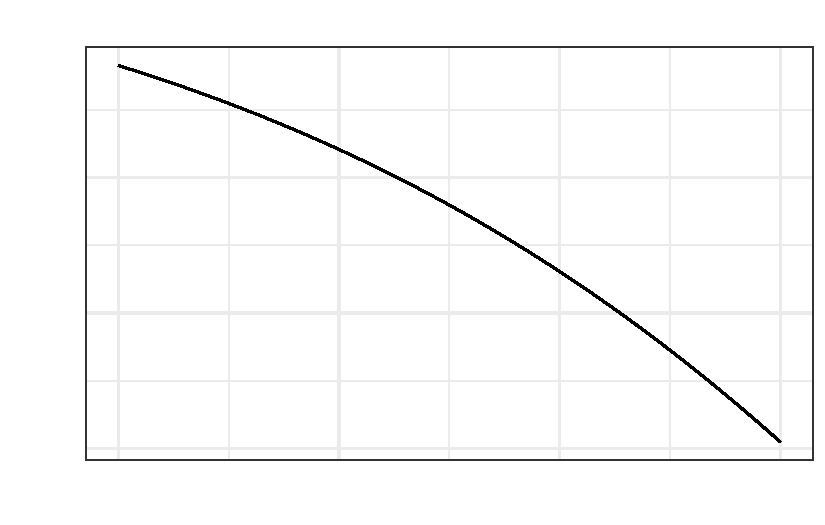
\includegraphics{main_files/figure-pdf/fig-line-plot-1.pdf}

}

\caption{\label{fig-line-plot}Probabilidade de não fumar}

\end{figure}

\begin{Shaded}
\begin{Highlighting}[]
\FunctionTok{ggplot}\NormalTok{(new\_df, }\FunctionTok{aes}\NormalTok{(}\AttributeTok{x =}\NormalTok{ distorcao\_idade\_serie, }\AttributeTok{y =}\NormalTok{ fit}\FloatTok{.2}\NormalTok{)) }\SpecialCharTok{+} \FunctionTok{geom\_line}\NormalTok{() }\SpecialCharTok{+} \FunctionTok{labs}\NormalTok{(}\AttributeTok{title =} \StringTok{"Probabilidade de fumar 1 ou 2 dias"}\NormalTok{, }\AttributeTok{y =} \StringTok{"Probabilidade"}\NormalTok{, }\AttributeTok{x =} \StringTok{"Distorção idade{-}série"}\NormalTok{) }\SpecialCharTok{+}\NormalTok{ abnt\_theme}
\end{Highlighting}
\end{Shaded}

\begin{figure}[H]

{\centering 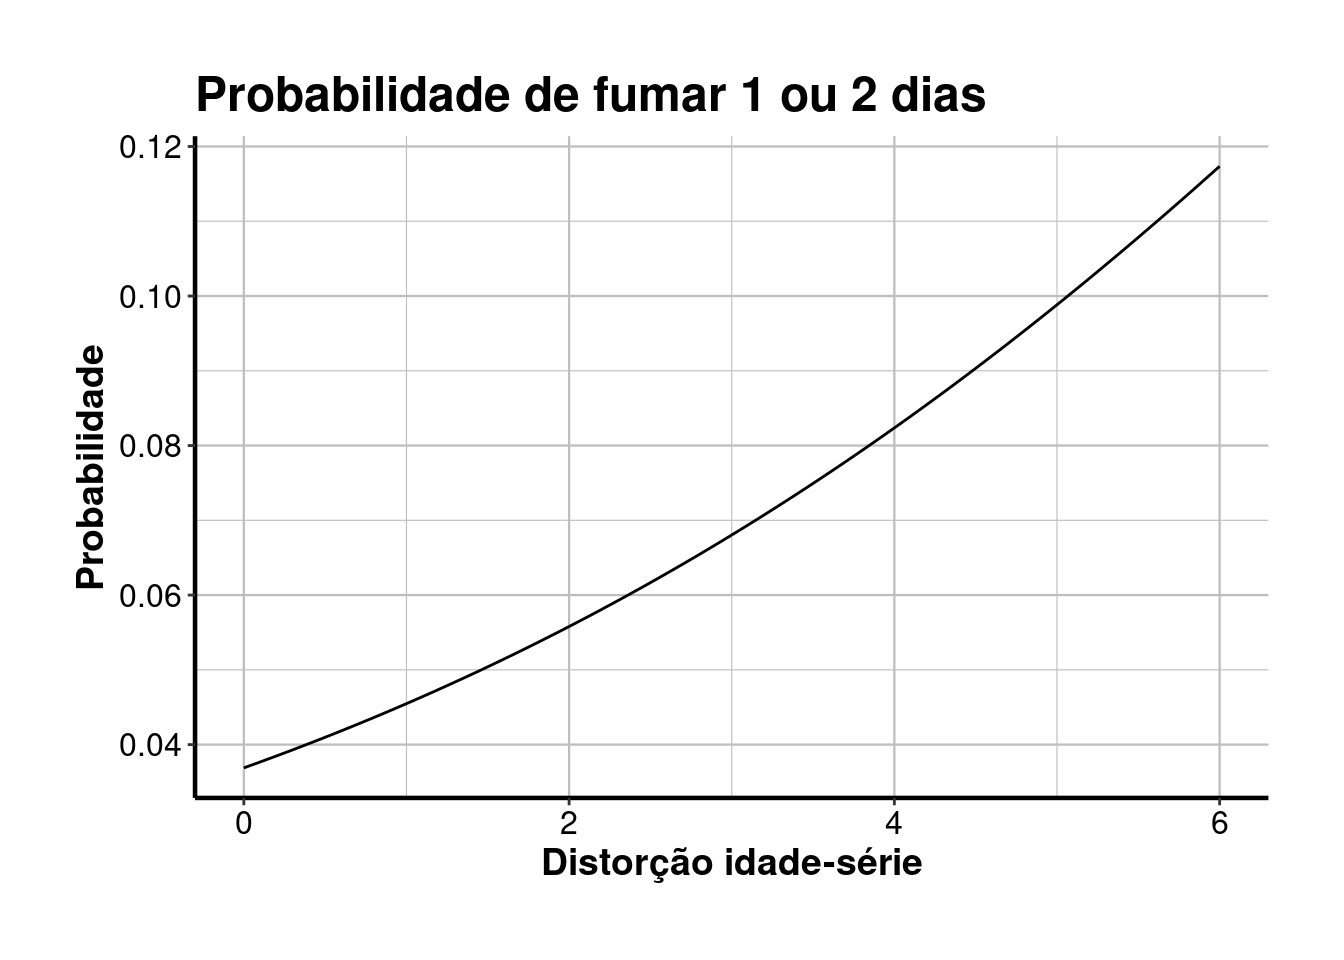
\includegraphics{main_files/figure-pdf/fig-line-plot2-1.pdf}

}

\caption{\label{fig-line-plot2}Probabilidade de fumar 1 ou 2 dias}

\end{figure}

\begin{Shaded}
\begin{Highlighting}[]
\FunctionTok{ggplot}\NormalTok{(new\_df, }\FunctionTok{aes}\NormalTok{(}\AttributeTok{x =}\NormalTok{ distorcao\_idade\_serie, }\AttributeTok{y =}\NormalTok{ fit}\FloatTok{.3}\NormalTok{)) }\SpecialCharTok{+} \FunctionTok{geom\_line}\NormalTok{() }\SpecialCharTok{+} \FunctionTok{labs}\NormalTok{(}\AttributeTok{title =} \StringTok{"Probabilidade de fumar 3 a 5 dias"}\NormalTok{, }\AttributeTok{y =} \StringTok{"Probabilidade"}\NormalTok{, }\AttributeTok{x =} \StringTok{"Distorção idade{-}série"}\NormalTok{) }\SpecialCharTok{+}\NormalTok{ abnt\_theme}
\end{Highlighting}
\end{Shaded}

\begin{figure}[H]

{\centering 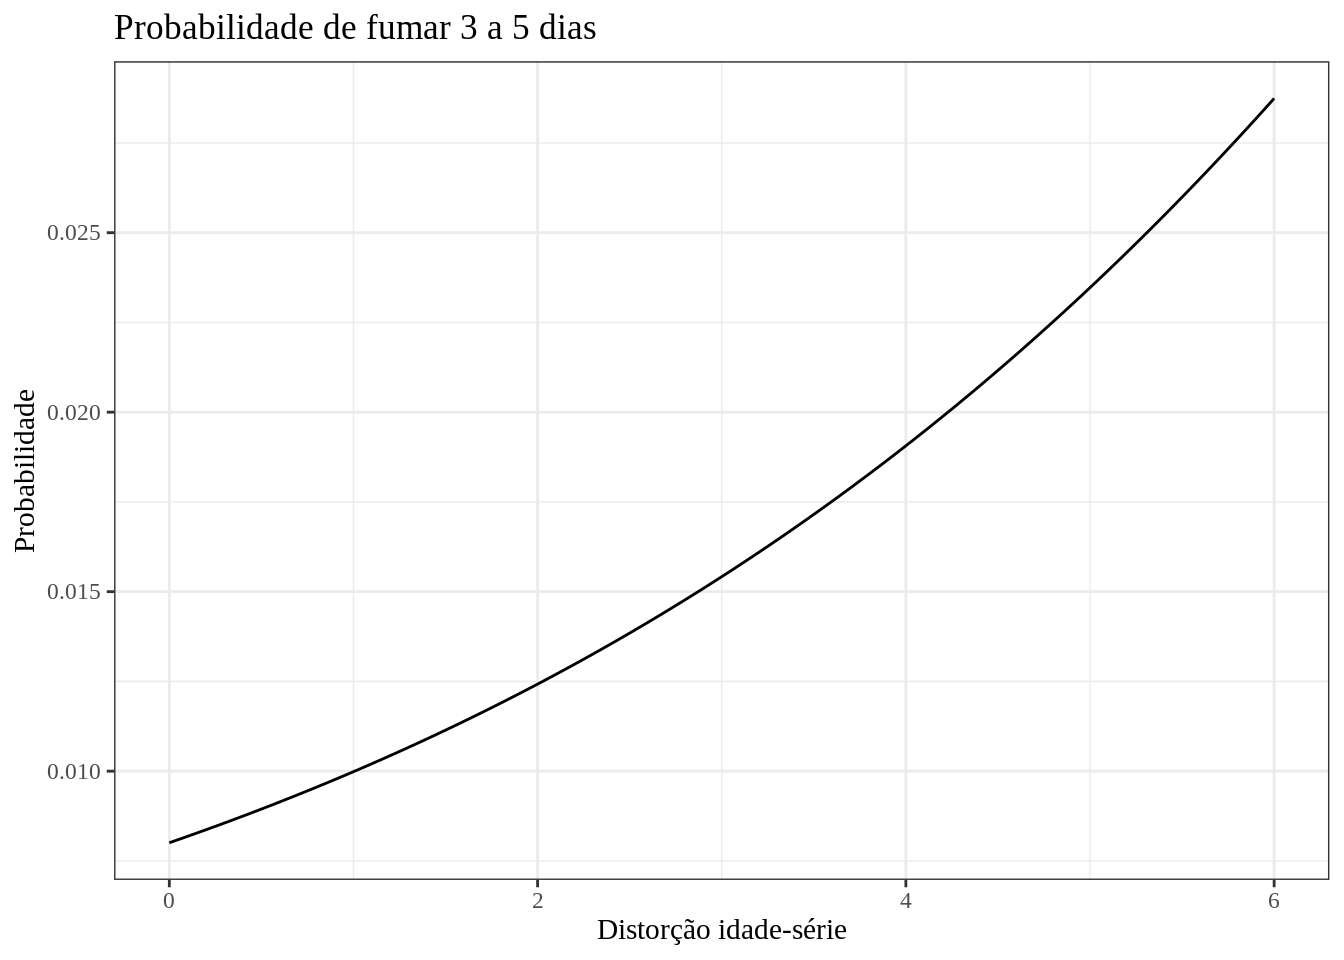
\includegraphics{main_files/figure-pdf/fig-line-plot3-1.pdf}

}

\caption{\label{fig-line-plot3}Probabilidade de fumar 3 a 5 dias}

\end{figure}

\begin{Shaded}
\begin{Highlighting}[]
\FunctionTok{ggplot}\NormalTok{(new\_df, }\FunctionTok{aes}\NormalTok{(}\AttributeTok{x =}\NormalTok{ distorcao\_idade\_serie, }\AttributeTok{y =}\NormalTok{ fit}\FloatTok{.4}\NormalTok{)) }\SpecialCharTok{+} \FunctionTok{geom\_line}\NormalTok{() }\SpecialCharTok{+} \FunctionTok{labs}\NormalTok{(}\AttributeTok{title =} \StringTok{"Probabilidade de fumar 6 a 9 dias"}\NormalTok{, }\AttributeTok{y =} \StringTok{"Probabilidade"}\NormalTok{, }\AttributeTok{x =} \StringTok{"Distorção idade{-}série"}\NormalTok{) }\SpecialCharTok{+}\NormalTok{ abnt\_theme}
\end{Highlighting}
\end{Shaded}

\begin{figure}[H]

{\centering 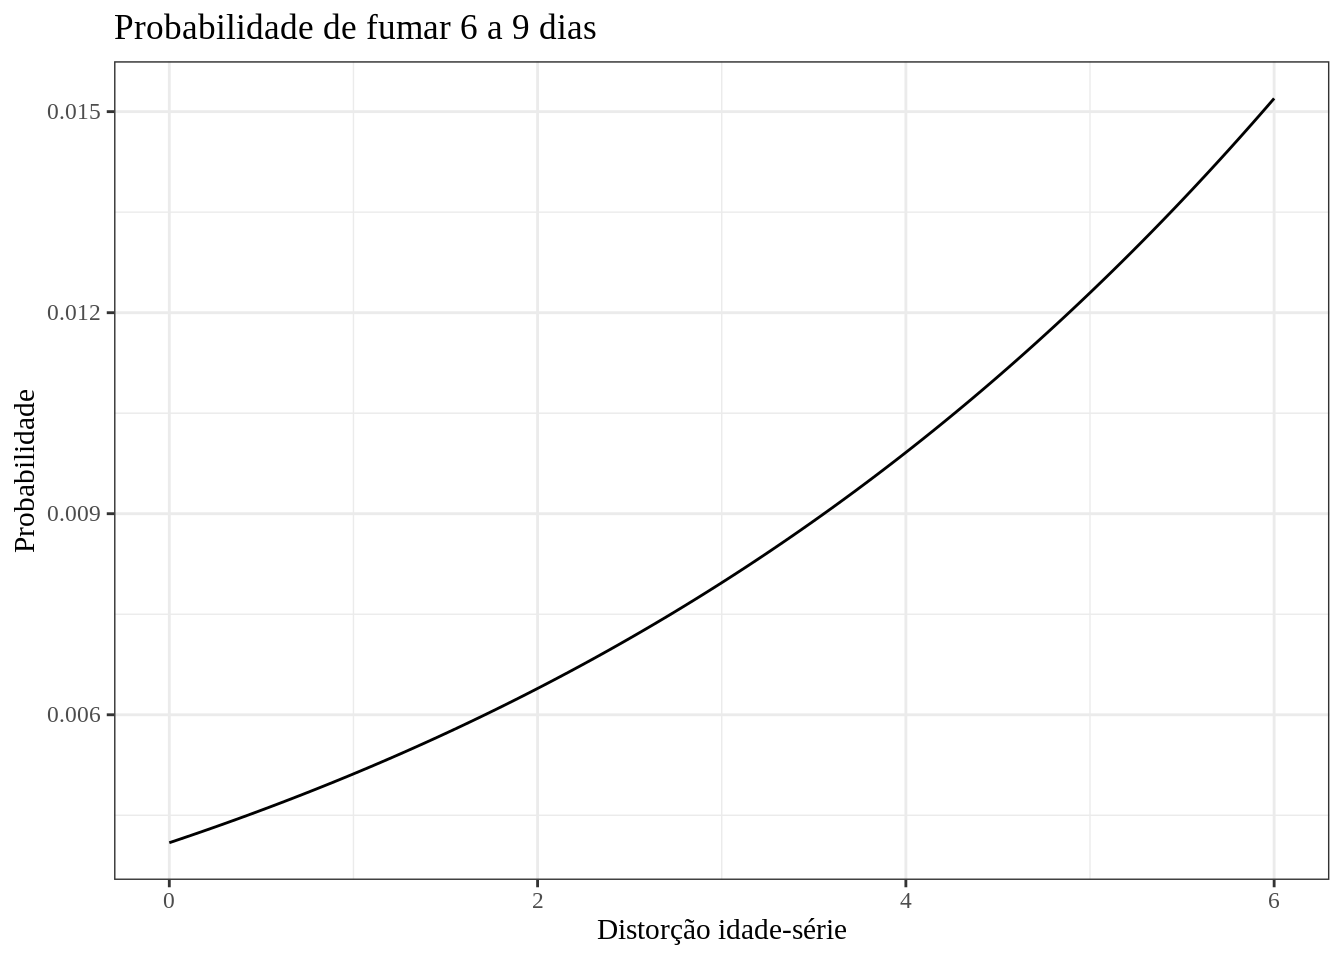
\includegraphics{main_files/figure-pdf/fig-line-plot4-1.pdf}

}

\caption{\label{fig-line-plot4}Probabilidade de fumar 6 a 9 dias}

\end{figure}

\begin{Shaded}
\begin{Highlighting}[]
\FunctionTok{ggplot}\NormalTok{(new\_df, }\FunctionTok{aes}\NormalTok{(}\AttributeTok{x =}\NormalTok{ distorcao\_idade\_serie, }\AttributeTok{y =}\NormalTok{ fit}\FloatTok{.5}\NormalTok{)) }\SpecialCharTok{+} \FunctionTok{geom\_line}\NormalTok{() }\SpecialCharTok{+} \FunctionTok{labs}\NormalTok{(}\AttributeTok{title =} \StringTok{"Probabilidade de fumar 10 a 19 dias"}\NormalTok{, }\AttributeTok{y =} \StringTok{"Probabilidade"}\NormalTok{, }\AttributeTok{x =} \StringTok{"Distorção idade{-}série"}\NormalTok{) }\SpecialCharTok{+}\NormalTok{ abnt\_theme}
\end{Highlighting}
\end{Shaded}

\begin{figure}[H]

{\centering 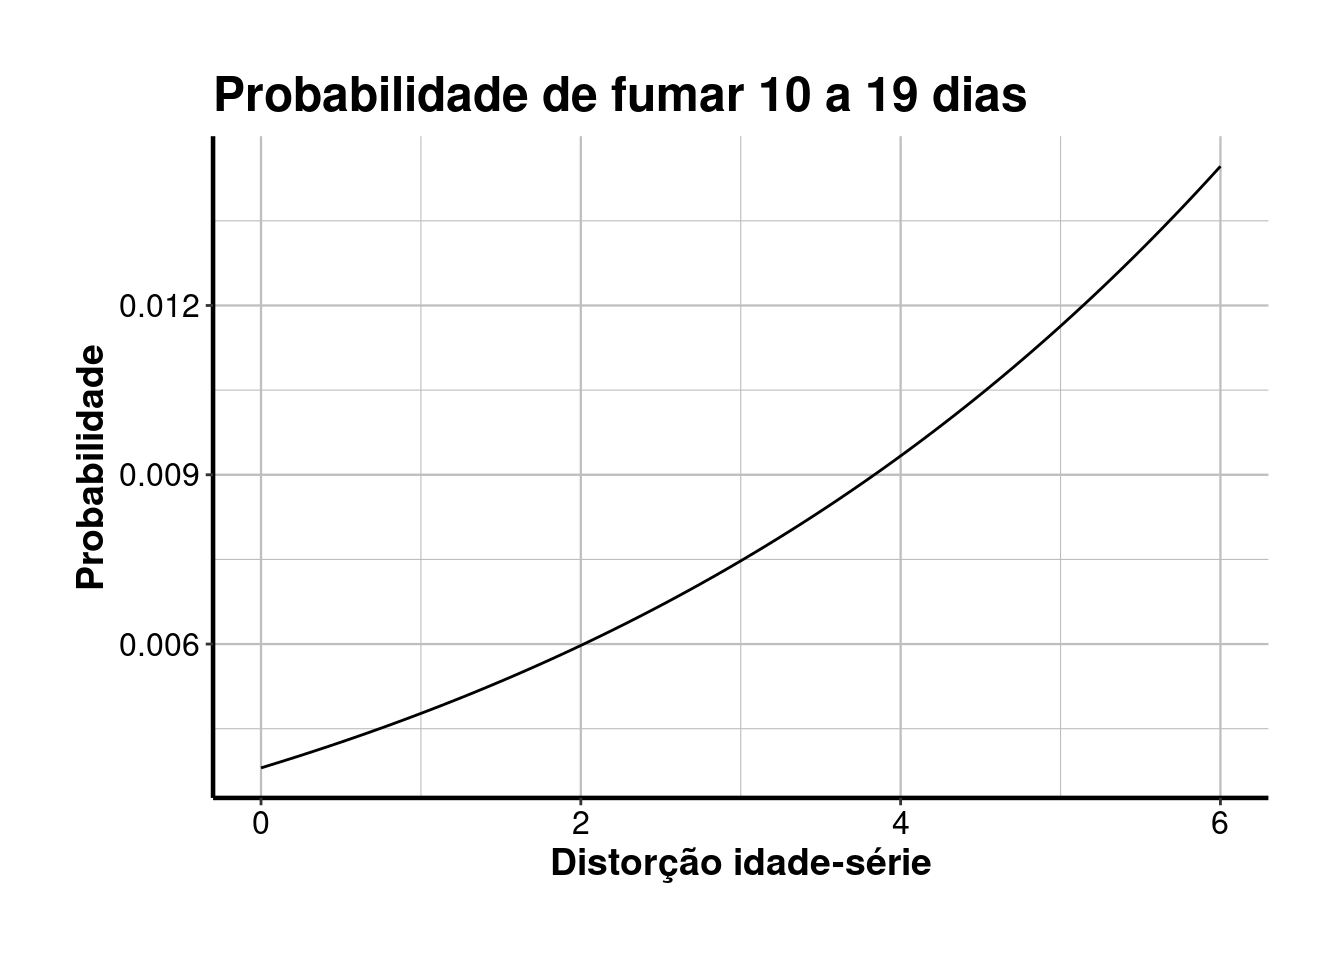
\includegraphics{main_files/figure-pdf/fig-line-plot5-1.pdf}

}

\caption{\label{fig-line-plot5}Probabilidade de fumar 10 a 19 dias}

\end{figure}

\begin{Shaded}
\begin{Highlighting}[]
\FunctionTok{ggplot}\NormalTok{(new\_df, }\FunctionTok{aes}\NormalTok{(}\AttributeTok{x =}\NormalTok{ distorcao\_idade\_serie, }\AttributeTok{y =}\NormalTok{ fit}\FloatTok{.6}\NormalTok{)) }\SpecialCharTok{+} \FunctionTok{geom\_line}\NormalTok{() }\SpecialCharTok{+} \FunctionTok{labs}\NormalTok{(}\AttributeTok{title =} \StringTok{"Probabilidade de fumar 20 a 29 dias"}\NormalTok{, }\AttributeTok{y =} \StringTok{"Probabilidade"}\NormalTok{, }\AttributeTok{x =} \StringTok{"Distorção idade{-}série"}\NormalTok{) }\SpecialCharTok{+}\NormalTok{ abnt\_theme}
\end{Highlighting}
\end{Shaded}

\begin{figure}[H]

{\centering 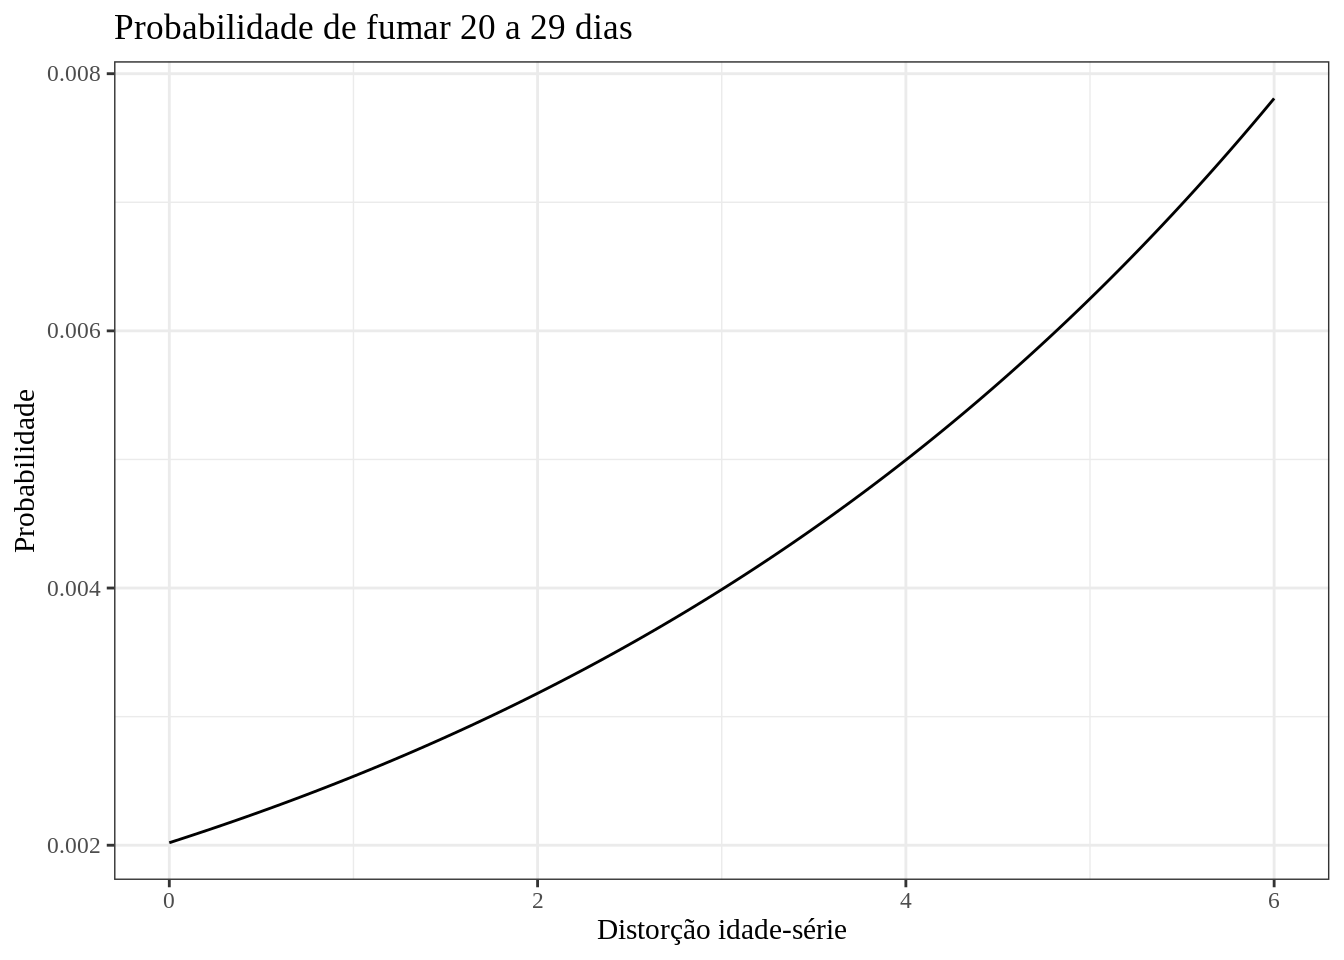
\includegraphics{main_files/figure-pdf/fig-line-plot6-1.pdf}

}

\caption{\label{fig-line-plot6}Probabilidade de fumar 20 a 29 dias}

\end{figure}

\begin{Shaded}
\begin{Highlighting}[]
\FunctionTok{ggplot}\NormalTok{(new\_df, }\FunctionTok{aes}\NormalTok{(}\AttributeTok{x =}\NormalTok{ distorcao\_idade\_serie, }\AttributeTok{y =}\NormalTok{ fit}\FloatTok{.7}\NormalTok{)) }\SpecialCharTok{+} \FunctionTok{geom\_line}\NormalTok{() }\SpecialCharTok{+} \FunctionTok{labs}\NormalTok{(}\AttributeTok{title =} \StringTok{"Probabilidade de fumar todos os dias"}\NormalTok{, }\AttributeTok{y =} \StringTok{"Probabilidade"}\NormalTok{, }\AttributeTok{x =} \StringTok{"Distorção idade{-}série"}\NormalTok{) }\SpecialCharTok{+}\NormalTok{ abnt\_theme}
\end{Highlighting}
\end{Shaded}

\begin{figure}[H]

{\centering 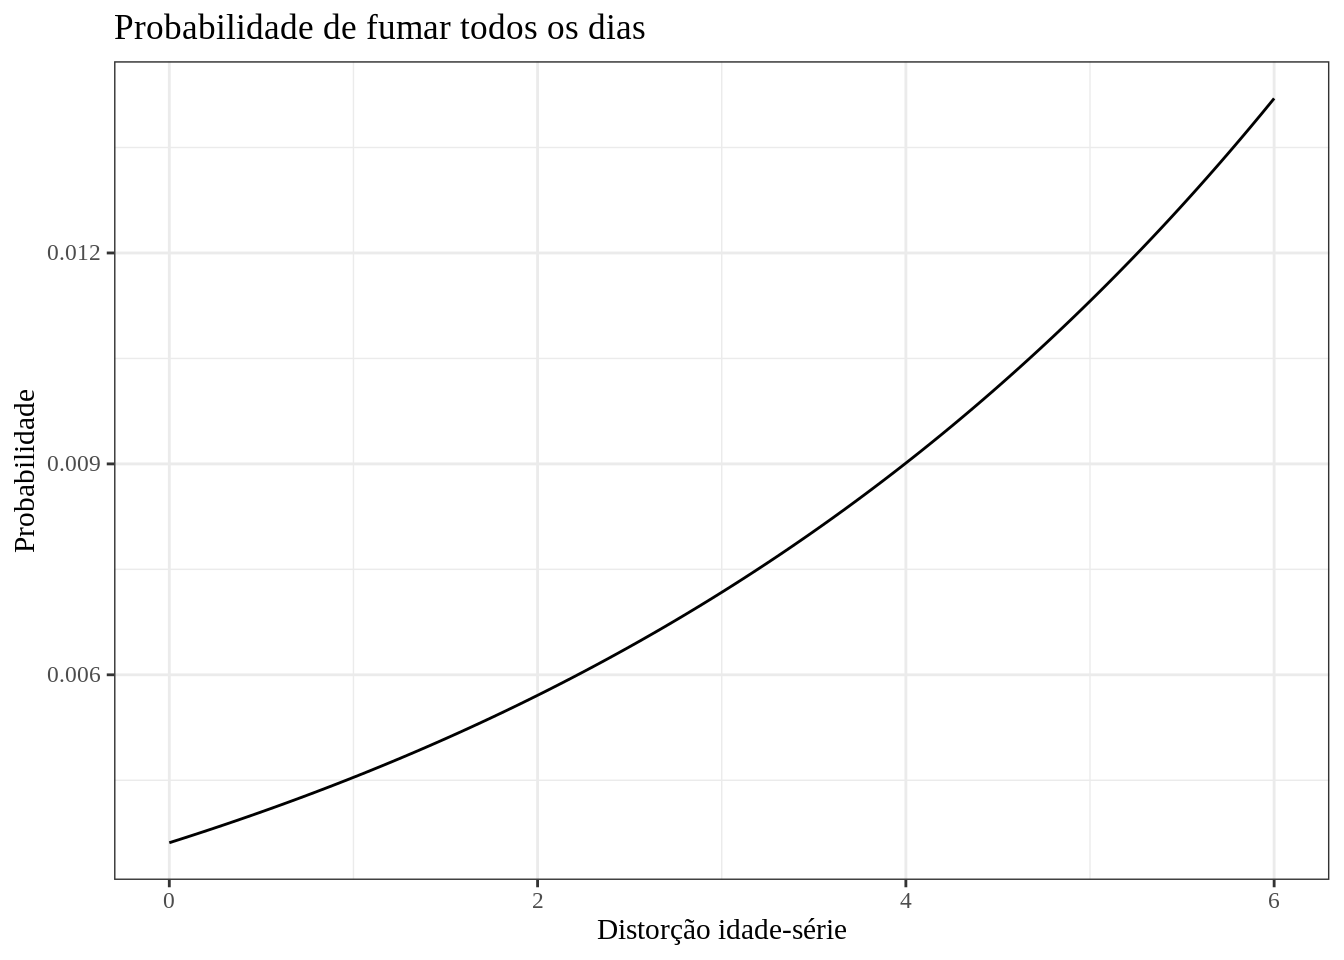
\includegraphics{main_files/figure-pdf/fig-line-plot7-1.pdf}

}

\caption{\label{fig-line-plot7}Probabilidade de fumar todos os dias}

\end{figure}

\hypertarget{referuxeancias}{%
\subsubsection{Referências}\label{referuxeancias}}

\hypertarget{refs}{}
\begin{CSLReferences}{0}{1}
\leavevmode\vadjust pre{\hypertarget{ref-agresti}{}}%
AGRESTI, A. \textbf{Categorical data analysis, Second Edition}. New
York, New York: Wiley, 2002.

\leavevmode\vadjust pre{\hypertarget{ref-bousquet}{}}%
BOUSQUET, C. A. H. et al.
\href{https://doi.org/10.1163/1568539X-00003431}{Determinants of
leadership in groups of female mallards}. \textbf{Behaviour}, v. 154, n.
4, p. 467--507, 2017.

\leavevmode\vadjust pre{\hypertarget{ref-christensen}{}}%
CHRISTENSEN, R. H. B. \textbf{ordinal --- Regression models for ordinal
data}. Disponível em:
\textless{}\url{http://www.cran.r-project.org/package=ordinal/}\textgreater.

\leavevmode\vadjust pre{\hypertarget{ref-oconnell}{}}%
O'CONNELL, A. A. \textbf{An illustration of multilevel models for
ordinal response data}. Data and context in statistics education:
Towards an evidence-based society. Proceedings of the Eighth
International Conference on Teaching Statistics (ICOTS8).
\textbf{Anais}...2010.

\leavevmode\vadjust pre{\hypertarget{ref-raudenbush}{}}%
RAUDENBUSH, S. W.; BRYK, A. S. \textbf{Hierarchical linear models:
Applications and data analysis methods}. {[}s.l.{]} sage, 2002. v. 1

\end{CSLReferences}



\end{document}
